\selectlanguage{french}
\Chapter{REVUE DE LA LITTÉRATURE}\label{sec:RevLitt}

\section{Matériaux composites}

Les matériaux structurels peuvent être divisés en 4 grandes classes: les métaux, les polymères, les céramiques et les verres, et les composites \cite{ashby2018materials}. 
Un matériau composite est un assemblage solide d'au moins deux phases hétérogènes aux propriétés différentes dans le but d'obtenir un matériau aux propriétés différentes des phases isolées. 
Les phases restent distinctes et séparées dans le matériau final \cite{Wikipedia_mat_comp}. 
Ces mélanges permettent d'obtenir des matériaux sur mesure avec des propriétés ajustées selon le besoin de l'application. 
Il est ainsi possible de produire des matériaux plus légers, plus résistants aux sollicitations mécaniques, plus conducteurs, plus rigides, avec une meilleure tenue en température ou toute autre propriété visée. 

Les matériaux composites modernes sont composés d'une matrice polymérique, métallique ou céramique, et d'un renfort sous forme de particules ou de fibres. 
Les matériaux composites sont divisés en catégories selon la nature des phases en présence. 
Si on exclut le béton, les composites à matrice polymérique représentent la majorité des composites produits industriellement. 
Comme matériaux de renforts utilisés, on retrouve une majorité de composites de fibres inorganiques telles que les fibres de verre ou les fibres de carbone et, dans une plus faible proportion, de composites à base de fibres polymériques telles que l'aramide (ex. : Kevlar, Nomex, etc.) ou le polyéthylène à très grande masse moléculaire (ex. : Dyneema, Spectra, etc. ). 
Ces fibres sont sélectionnées pour leur très grande résistance spécifique et leur module de Young élevé. 
Les composites modernes utilisent une grande variété de fibres aux propriétés variées (Fig. \ref{gibson2}). 
Les fibres sont disponibles commercialement sous la forme de fibres courtes, de rouleaux de fibres unidirectionnelles ou de toiles tissées. 

\begin{figure}
	\centering
	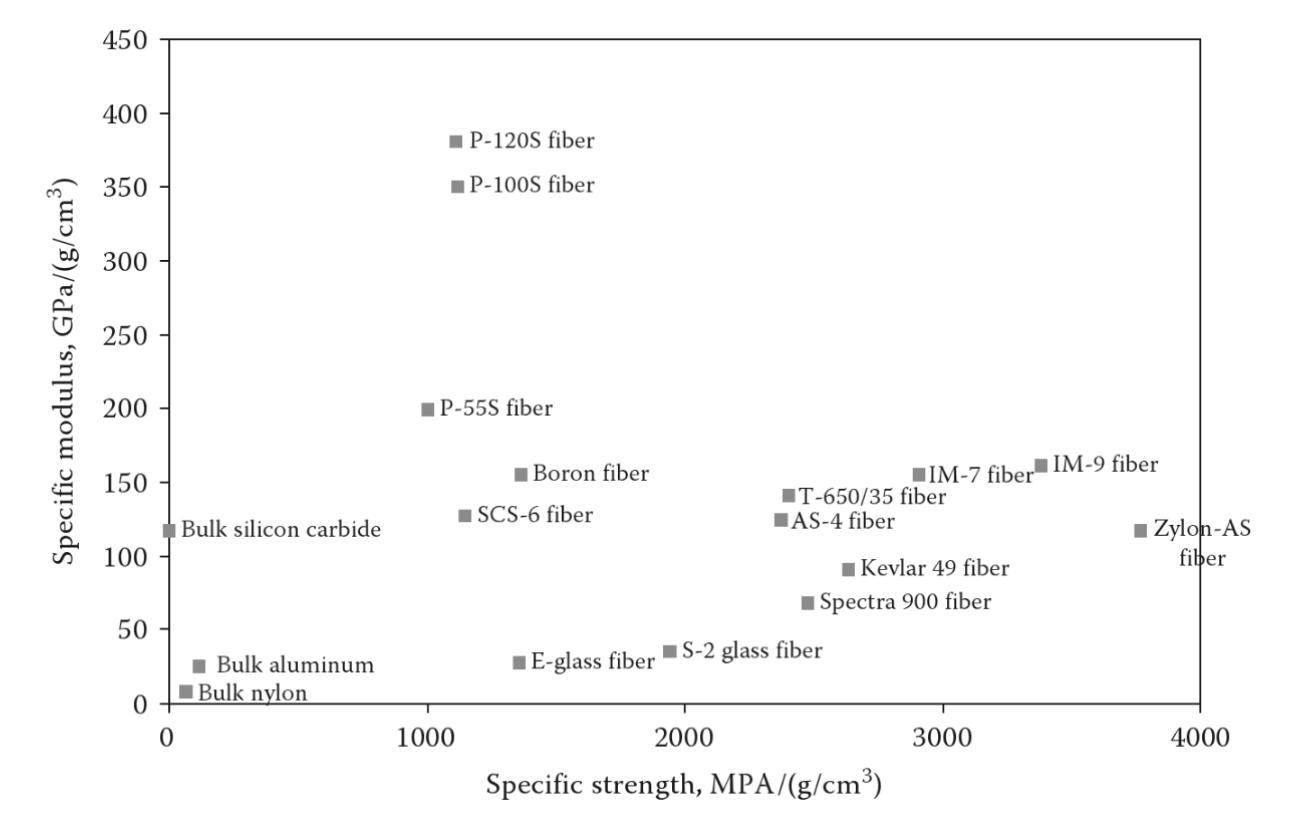
\includegraphics[width=0.9\textwidth]{gibson2}
	\caption{Comparaison des fibres utilisées pour les composites modernes (tirée de \cite{Gibson2011}, reproduction avec autorisation)}
	\label{gibson2}
\end{figure}

En ce qui concerne la matrice, les développements initiaux des composites à matrice polymérique ont été réalisés avec des polymères thermodurcissables. 
Ces derniers ont été favorisés au départ en raison de la possibilité de les employer à l'état liquide à pression ambiante, avant la polymérisation, pour imprégner les fibres \cite{Chatain2015}. 
C'est pour cette raison qu'encore aujourd'hui les composites à matrice thermodurcissable occupent la majorité du marché des composites à matrice polymérique. 

\FloatBarrier
\subsection{Performances}

Les performances mécaniques des composites proviennent de la combinaison des fibres et de la matrice qui les supportent. 
Malgré leur très faible densité, les fibres possèdent des modules d'élasticité et des résistances à la traction très élevés en comparaison avec les propriétés des matériaux traditionnels tels que les aciers alliés ou l'aluminium \cite{Hull2001}.
Cependant, les fibres offrent très peu de résistance à la compression dans leur axe en raison de leur géométrie et sont incapables de redistribuer la charge entre elles sans l'aide d'un support. 
En combinant les fibres rigides à une matrice leur offrant un support et permettant de transférer les charges, on obtient un matériau aux propriétés fortement dépendantes de l'orientation. 
Les matériaux composites à fibres continues sont très résistants face aux sollicitations orientées selon le sens des fibres, mais ils sont très sensibles aux sollicitations en dehors de cet axe. 
Une déviation de plus de 5° dans l'orientation de la force produit une forte dégradation des performances \cite{Hull2001}. 
Il est donc important lors de la fabrication de conserver l'orientation des fibres afin d'obtenir des propriétés mécaniques optimales. 
De plus, même si chaque pli de composite est sensible aux sollicitations en dehors de son axe principal, il est possible de superposer une série de plis avec différentes orientations afin que le laminé composé possède de meilleures propriétés selon certains axes définis. 

En ce sens, le développement de pièces en composite doit prendre en compte la nature directionnelle des propriétés des composites, puisqu'un impact sur les résultats sera observable lors de l'évaluation de la résistance aux chargements mécaniques. 
Néanmoins, la faible densité des matériaux composites permet de réduire le poids global des structures en maintenant les niveaux de performances. 

Un autre avantage de la nature hétérogène des composites réside dans leur résistance à la propagation des fissures. 
Contrairement aux métaux qui n'offrent pas de frontières à la propagation des fissures, la présence de fibres au travers des fissures permet de maintenir une intégrité mécanique des pièces. 
Tandis que la matrice polymérique peut fissurer et se déformer pour absorber une partie de l'énergie de déformation, les fibres résistent encore un moment en ralentissant la vitesse de propagation des fissures \cite{Hull2001}. 

\subsection{Composites à matrice thermoplastique}

Les composites à matrice thermoplastique ont commencé à être considérés sérieusement durant les années 1980 pour améliorer la durabilité et la résilience aux impacts à basse vitesse des composites \cite{asmhandbook21}. 
Même si le marché continue d'utiliser en grande quantité les matrices thermodurcissables, les compagnies aéronautiques telles qu'ArianeGroup convertissent de plus en plus leurs procédés de fabrication pour utiliser les composites thermoplastiques. 
Du côté de l'automobile également, afin de rencontrer les cibles de consommation de carburant américaines et européennes, les manufacturiers intègrent un volume croissant de composites à leurs produits afin d'en réduire la masse. 
Les composites à matrice thermoplastique occupent un rôle central dans cette transition \cite{CompositesWorld2019_market2020}. 

En plus de leur plus grande résilience, les composites à matrice thermoplastique sont moins sensibles aux contaminants et à leur environnement que les composites à matrice thermodurcissable, et ce, autant durant leur service ainsi que lors de leur mise en forme. 
Puisque les composites à matrice thermoplastique sont déjà totalement polymérisés, la présence de solvants ou de graisse n'affecte pas le processus de polymérisation \cite{cogswell1992}. 
Les composites thermoplastiques ont également une plus faible sensibilité à l'humidité.  
La polymérisation complète des matrices thermodurcissables nécessite des durées de plusieurs heures suivies de traitements de cuisson, souvent à l'autoclave, pour terminer la réaction. 
La mise en forme à l'autoclave des composites à matrice thermodurcissable, pour le domaine de l'aéronautique, nécessite une grande quantité d'énergie et d'espace. 
Les dimensions des autoclaves doivent être suffisantes pour contenir par exemple des pièces du fuselage ou encore des segments d'ailes. 
Même si la puissance requise pour chauffer une pièce en composites à matrice thermoplastique est plus élevée lors de sa mise en forme, la courte durée de cette opération réduit grandement les besoins en énergie comparativement à celle nécessaire à la cuisson des composites thermodurcissables sur une longue durée. 
L'élimination du temps nécessaire à la polymérisation et à la cuisson permet de raccourcir grandement les temps de production et ainsi de multiplier la cadence de production. 
Finalement, puisque les thermoplastiques peuvent être refondus, il est possible de réparer les composants à la suite de fissures n'ayant pas cassé les fibres ou encore de les recycler en fin de vie utile. 

\subsection{Mise en forme}

Contrairement aux composites à matrice thermodurcissable qui doivent être moulés directement à leur forme finale, les composites à matrice thermoplastique ont la possibilité d'être fondus à plusieurs reprises. 
Les différentes méthodes de mise en forme des composites à matrice thermoplastique sont principalement des variations quant aux méthodes de chauffe et de mise en place des matériaux. 

Les principales méthodes de fabrication sont l'enroulement filamentaire, la déposition de ruban, le moulage par compression dans un moule rigide ou flexible, la mise en forme par diaphragme dans une presse ou en autoclave, l'emboutissage, le laminage, l'extrusion par tirage et le transfert de résine \cite{asmhandbook21, campbell2003}.  

La sélection d'une méthode de mise en forme repose sur le type de géométrie à réaliser, le type de fibre qui doit être utilisé et la nature du polymère. 
Par exemple, les procédés d'enroulement filamentaire ou encore de mise en forme par déposition de ruban ne permettent pas de fabriquer des composites avec des toiles tissées. 
Ces procédés ont la particularité d'employer des rubans de fibres unidirectionnelles déposés de façon linéaire. 
Il est cependant possible de changer la direction de déposition lors des passages subséquents pour obtenir un composite avec des couches orientées différemment. 
Dans le même ordre d'idées, le procédé de transfert de résine ne peut être appliqué qu'aux thermoplastiques pouvant être injectés sous forme de monomères qui polymériseront ensuite dans la pièce tels que le polyamide-6 anionique (APA-6) \cite{Rijswijk2006} ou certaines résines acryliques récemment développées \cite{Penumadu2019,Murray2019}. 

Notre partenaire industriel a développé un procédé d'enroulement filamentaire avec un chauffage par laser pour la fabrication des réservoirs \cite{Krzeminski2014}. 
Le procédé développé pour joindre les plaques de composites à l'élastomère devra donc être compatible avec ce type de pièces. 

\subsection{Jonction des pièces en composite}

En raison de la nature directionnelle des propriétés des matériaux composites,la jonction effectuant le transfert de charge entre les composants mécaniques ne peut être conçue comme pour les matériaux isotropes. 
Les jonctions entre pièces de composites présentent des discontinuités dans la structure même du matériau. 
De façon plus prononcée que pour les pièces réalisées à l'aide de matériaux isotropes, les jonctions représentent des zones critiques lors de la conception de structures en composite. 
En raison de la flexibilité des processus de mise en forme, il est possible de réduire le nombre de jonctions en produisant des composants aux géométries plus complexes. 
Parfois, une seule pièce en composite peut remplacer tout un assemblage de pièces et ainsi sauver des coûts \cite{KarenMas_CW2004}. 

Les méthodes employées pour réaliser des jonctions entre les pièces en composite peuvent être classifiées en deux grandes catégories. 
\begin{enumerate}
	\item Les jonctions ponctuelles qui causent un transfert de charge qui peut être localisé en un point. 
	Cette catégorie englobe les liaisons avec des rivets et le soudage point à point. 
	\item Les méthodes permettant plutôt un transfert de charge sur une surface. 
	Cette seconde catégorie englobe des procédés tels que le collage ou le soudage. 
\end{enumerate}
Afin de favoriser un bon transfert des charges mécaniques, pour les applications structurelles où les pièces ne peuvent pas être combinées afin d'éliminer les jonctions, les joints de la seconde catégorie sont fortement conseillés \cite{campbell2003}. 

Les composites thermodurcissables sont limités dans les options d'assemblage. 
Il est possible de les assembler par co-consolidation, collage ou assemblage mécanique à l'aide de boulons ou de rivets.
Dans le cas des composites à matrice thermoplastique, un plus large éventail de méthodes de soudage s'ajoute aux méthodes déjà disponibles pour les composites thermodurcissables \cite{campbell2003}. 
Puisque le collage de composites à matrice thermoplastique produit des joints moins résistants que pour les composites à matrice thermodurcissable --- en raison de la nature des polymères \cite{campbell2003} --- et que les procédés de soudage sont moins sensibles aux contaminants, ces derniers sont préférés pour l'assemblage des composants. 

\section{Reptation des polymères thermoplastiques}

La reptation des chaînes est un phénomène clé pour la compréhension de l'évolution du comportement mécanique des jonctions soudées. 
Pendant le procédé de soudage, lors de la mise en contact des faces à joindre, les chaînes de polymères mobiles diffusent entre les pièces et on observe progressivement une homogénéisation de la soudure et la disparition de la frontière entre les pièces (Fig. \ref{fig:polymer_diffusion}). 
Cette diffusion des chaînes se produit principalement en deux étapes. 
\begin{enumerate}
	\item Développement du contact intime entre les adhérents.
	\item Cicatrisation de l'interface.
\end{enumerate}

\begin{figure}[h]
	\centering
	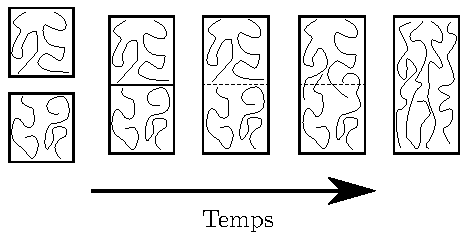
\includegraphics[scale=1.2]{welding_chain_diffusion.pdf}
	\caption{Diffusion des chaînes de polymères durant le soudage : a) état initial, b) mise en contact des faces, c) formation du contact intime entre les faces, d) diffusion des chaînes de polymères au travers de l'interface et e) disparition de l'interface. }
	\label{fig:polymer_diffusion}
\end{figure}

Avant même que la diffusion des chaînes ne puisse prendre place, les faces en contact doivent atteindre un état de contact intime. 
Durant cette étape, les surfaces se conforment les unes aux autres, mais la diffusion des chaînes de polymères n'a pas encore débuté. 
La question de contact intime a été abordée très tôt dans le développement des composites à matrice thermoplastique en raison de la nécessité de consolider les couches lors de la fabrication des pièces. 
Les équations développées pour l'atteinte de cet état prennent en compte la rugosité de la surface à l'aide de paramètres géométriques ($a^*$ et $w^*$), la pression de contact ($P_{app}$) et la viscosité de la matrice polymérique ($\mu _{mf}$). 
Les premiers modèles simplifiaient la surface en une série de rectangles idéalisés d'aire constante, mais dont la hauteur et la largeur varient en fonction du temps \cite{Lee1987}. 
En intégrant la variation de la pression et de la viscosité sur le temps depuis la mise en contact ($t_c$), on arrive à l'équation suivante décrivant le degré de contact intime ($D_{ic}$) \cite{Mantell1992a} : 

\begin{equation}
D_{ic} \approx \frac{1}{w^*} \left[ a^* \int_{0}^{t_c} \frac{P_{app}}{\mu _{mf}} \, dt \right]^{\frac{1}{5}}
\label{eq:contact_intime}
\end{equation}

Les modèles basés sur des rectangles idéalisés sont incapables de prédire le comportement depuis des mesures directes de la rugosité des interfaces et nécessitent des paramètres d'ajustement obtenus à la suite d'essais en laboratoire \cite{Yang2001}. 
Une autre génération de modèles tente plutôt de représenter la surface comme une série de rectangles de tailles diverses parfois semblables à une fractale dont les propriétés peuvent être reliées à des mesures de rugosité des surfaces \cite{Yang2001,Yang2002}. 
Dans ces modèles, le polymère est écrasé jusqu'à ce que tous les rectangles d'aire constante forment une frontière unique. 
À partir de données de rugosité, Yang et Pitchumani ont pu établir un modèle montrant une évolution rapide du critère de contact intime suivi d'un ralentissement à l'approche du plein contact \cite{Yang2001}. 
Dans des conditions isothermes à \SI[locale=FR]{350}{\celsius} avec des pressions de 0,67 et \SI[locale=FR]{1,63}{\mega\pascal}, le contact intime est totalement atteint avec des temps respectivement de \SI[locale=FR]{100}{\second} et de \SI[locale=FR]{40}{\second} pour des laminés en Polyétheréthercétone (PEEK). 
Une hausse de la température ou de la pression diminue très rapidement le temps nécessaire pour atteindre la condition de contact intime \cite{Yang2002}. 

La seconde étape du développement de la jonction entre les pièces est la cicatrisation de l'interface. 
Ce phénomène se produit par la diffusion des chaînes de polymères au travers de l'interface entre un même polymère ou des polymères compatibles \cite{Jud1981b}. 
La reconfiguration des chaînes dans le polymère se produit par un phénomène de reptation et de mouvement brownien qui a été conceptualisé, pour les polymères fondus, assez tôt \cite{DeGennes1971,Edwards1978b,Klein1978,Daoud1979}. 
La cicatrisation par transfert des chaînes de polymères au travers de l'interface peut se produire lorsque des polymères amorphes compatibles sont chauffés au-dessus de leur température de transition vitreuse et qu'ils sont en contact \cite{Jud1981a,Prager1981a}. 
La cicatrisation se produit par le mouvement stochastique de l'extrémité des chaînes entre deux pièces en contact et entraîne une reconfiguration des chaînes. 
Cette dernière entraîne également la formation d'enchevêtrements de chaînes au travers de l'interface \cite{Wool1983}
La diffusion des chaînes entraîne la disparition progressive de la démarcation entre les pièces en contact. 
Le temps requis pour cicatriser une fissure a été défini comme étant le temps nécessaire pour que les molécules adjacentes à la fissure diffusent à mi-chemin \cite{Prager1981a}.
Selon la nature du polymère, son poids moléculaire, la température et la pression, le processus de cicatrisation peut se produire en quelques minutes ou peut nécessiter plusieurs heures voire même des jours \cite{Prager1981a}. 
On nomme le temps de reptation ($t_r$) le temps que prend une chaîne de polymère pour quitter totalement sa configuration d'origine et atteindre une nouvelle configuration géométrique. 
Dans le cas d'une soudure où l'ensemble de la surface n'est pas à une température constante, la cicatrisation commence à se produire progressivement dans les sections ayant déjà atteint le contact intime. 

Le temps de reptation est un paramètre clé pour évaluer la vitesse du phénomène de diffusion des chaînes de polymères. 
Pour les polymères amorphes, on peut citer les travaux de Wool \cite{Wool1983,Wool1989}. 
Ces derniers traitent de l'évolution des propriétés mécaniques durant la phase de transition vers la diffusion complète des chaînes de polymères en condition isotherme. 
Il dénote entre autres que la quantité d'énergie nécessaire pour séparer des interfaces dépend de quatre paramètres : \begin{inparaenum}[(1)]
	\item le temps ($t$), 
	\item la température ($T$), 
	\item la pression ($P_{app}$) et
	\item la masse moléculaire ($M$). 
\end{inparaenum}
Ce dernier paramètre est directement lié au temps de reptation tel que \cite{DeGennes1971}: 

\begin{equation}
t_r \approx M^3
\end{equation}

Wool introduit également plusieurs relations dynamiques décrivant le déplacement des chaînes de polymères en fonction du temps \cite{Wool1983,Wool1989}. 
Une première relation introduite est la longueur moyenne des chaînes mineures ayant traversé l'interface en fonction du temps ($l(t)$). 
Les chaînes mineures sont définies comme étant la section des chaînes ayant quitté le tube initial dans lequel la chaîne complète était initialement contenue. 
Les chaînes mineures débutent depuis l'extrémité des chaînes et croissent progressivement tout au long de la chaîne jusqu'à se rejoindre au milieu. 
On peut conceptualiser le mouvement des chaînes mineures comme étant un mouvement de marche aléatoire. 
Depuis la longueur moyenne des chaînes mineures, la distance moyenne d'interpénétration des monomères en fonction du temps ($\chi(t)$) peut être évaluée. 
Ces deux paramètres évoluent selon deux échelles de temps distinctes. 

\begin{equation}
l(t) \propto t^{1/2} M^{-1/2}
\end{equation}

\begin{equation}
\chi(t) \propto t^{1/4} M^{-1/4}
\end{equation}

L'impact de la température sur le temps de reptation peut être évalué à l'aide d'une équation d'Arrhenius où les paramètres $A_r$ et $B_r$  doivent être évalués expérimentalement \cite{Bastien1991,Ageorges1998}. 

\begin{equation}
t_r = B_r \, exp \left( \frac{A_r}{T} \right)
\end{equation}

En condition isotherme et pour un temps de reptation donné, les propriétés mécaniques ($\sigma$ et $\sigma_{\infty}$) évoluent, en fonction du temps ($t$), de façon non linéaire où le degré de cicatrisation ($D_{h}$) est estimé tel que \cite{F.Yang2002} : 

\begin{equation}
D_h \left( t \right) = \frac{\sigma}{\sigma_{\infty}} \propto \left( \frac{t}{t_r} \right)^{1/4}
\end{equation}

Autrement, en définissant les propriétés mécaniques à un temps infini ($\sigma_{\infty}$) telles que \cite{Wool1983} :

\begin{equation}
\sigma_{\infty} \propto M^{1/2}
\end{equation}

et en observant que les propriétés mécaniques évoluent, pour des temps inférieurs au temps de reptation, telles que \cite{Wool1983} :

\begin{equation}
\sigma \propto \left( \frac{t}{M} \right) ^{1/4}
\end{equation}

on obtient, pour la période où le temps ($t$) est inférieur au temps de reptation ($t_r$), une estimation de l'évolution les propriétés mécaniques de la soudure \cite{Wool1983} : 

\begin{equation}
\frac{\sigma}{\sigma_{\infty}} \propto t^{1/4} M^{-3/4}
\end{equation}

D'autres chercheurs (tels que Bastien, Yang et Ageorges) ont développé des équations décrivant l'évolution de la cicatrisation pour tenir compte de conditions non isothermes en discrétisant les phénomènes de contact intime et d'autohésion en fonction du temps  \cite{Bastien1991,F.Yang2002,Ageorges1998}. 

En se basant sur des données expérimentales provenant d'essais en condition isotherme réalisés dans le but d'estimer les temps de reptation en fonction de la température, Bastien a pu prévoir la résistance obtenue après un soudage en condition non isotherme, pour des jonctions entre des adhérents en polyétherimide (PEI) \cite{Bastien1991}. 
Les modèles développés par Bastien utilisent des critères basés sur longueur moyenne des chaînes mineures ayant traversé l'interface en fonction du temps ($l(t)$) et sur la distance moyenne d'interpénétration des monomères en fonction du temps ($\chi(t)$) développés par Wool \cite{Wool1983}. 
Le modèle de Bastien basé sur la distance moyenne d'interpénétration obtient des temps de reptation du même ordre de grandeur que les temps de reptation évalués expérimentalement (Tab. \ref{tab:temps_de_reptation_Bastien}). 
Le modèle basé sur la longueur des chaînes mineures ayant traversé l'interface donne des temps de reptation qui divergent des mesures expérimentales. 
Les résultats obtenus avec le paramètre d'interpénétration ont des marges d'erreur d'environ 20\%, mais confirment la possibilité d'obtenir des soudages de qualité avec des temps de mise en forme courts.

\begin{table}[h]
	\centering
	\caption{Évaluation expérimentale des temps de reptation et comparaison avec les résultats des modèles (traduit de \cite{Bastien1991})}
	\label{tab:temps_de_reptation_Bastien}
	\begin{tabular}{@{}lcccc@{}}
		\toprule
		& \multicolumn{1}{l}{} &          \multicolumn{3}{c}{Temps de reptation}          \\
		Type d'essai         &          Température &      Résultats &          Critère &  Critère \\
		&                      &   expérimentaux & $\chi(t)$ & $l(t)$ \\
		&      [\si{\celsius}] & [\si{\second}] &   [\si{\second}] &       [\si{\second}] \\ \midrule
		Moulage à la presse  &                  230 &        300 880 &          510 000 &            5 400 000 \\
		Essais de fluage     &                  250 &           4 800 &             5 446 &               99 131 \\
		Mesures en rhéologie &                  270 &          1 - 8 &               81 &                 2 437 \\ \bottomrule
	\end{tabular}%
\end{table}

Un modèle subséquent est parvenu à améliorer les prédictions de temps de cicatrisation pour les conditions de variations rapides de température et permet d'évaluer avec plus de précision l'état d'une interface soudée \cite{F.Yang2002}. 
Les équations de développement du contact intime et du phénomène de cicatrisation ont été mis en application avec des résultats probants pour élaborer une fenêtre d'opération pour le soudage de composites à matrice thermoplastique~\cite{Ageorges1998}. 

La littérature n'est pas aussi développée en ce qui concerne les thermoplastiques semi-cristallins. 
Cependant, certains travaux ont permis de démontrer l'importance de la co-cristallinité et de la température sur la possibilité d'obtenir un soudage entre thermoplastiques semi-cristallins  \cite{Xue1998,Smith2001}. 
Le taux de cristallinité a également un grand impact sur la possibilité de souder des pièces. 
Les cristaux présents dans les adhérents semi-cristallins affectent la facilité avec laquelle les chaînes de polymères peuvent migrer à l'interface \cite{Jarrousse2004}. 
Un taux de cristallinité élevé crée des entraves au déplacement des chaînes en dessous de la température de fusion tandis qu'un échantillon faiblement cristallin possède des zones amorphes qui peuvent migrer et interdiffuser sous la température de fusion. 
Lors de la fusion des cristaux, la possibilité de former des cristaux en co-cristallinité qui unissent les deux phases est un facteur important à considérer \cite{Smith2001,Zanetto2001}. 
Plus la température est élevée, plus la soudure pourra se développer jusqu'à atteindre la résistance normale du polymère. 

\section{Soudage des composites à matrice thermoplastique}

Les composites à matrice thermoplastique, contrairement aux composites à matrice thermodurcissable, ont la possibilité d'être fondus pour modifier leur forme. 
Cette particularité leur permet également d'être pliés ou emboutis pour former des géométries plus complexes à partir de plaques planes ou encore de les assembler par soudage. 
Lors du soudage, les pièces à joindre sont fondues ou chauffées à l'interface, pressées ensemble et finalement consolidées pour obtenir une seule pièce continue. 
L'absence de transition dans le matériau a ouvert la porte à la certification des pièces obtenues pour le domaine de l'aviation \cite{Gardiner2018}. 

\begin{figure}[h]
	\centering
	\resizebox{0.75\textwidth}{!}{
		\tikzset{
	basic/.style  = {draw, text width=6cm, drop shadow, rectangle},
	root/.style   = {basic, rounded corners=2pt, thin, align=center,
                   fill=gray!30},
	level 2/.style = {basic, rounded corners=5.5pt, thin,align=center, fill=gray!10,
                   text width=8em},
	level 3/.style = {basic, thin, align=left, fill=white, text width=6.em}
}


\begin{tikzpicture}[
	level 1/.style={sibling distance=45mm},
	edge from parent/.style={->,draw},
	>=latex,
	scale=0.9,
	level distance=1.8cm]

% root of the the initial tree, level 1
\node[root] {Procédés de soudage}
% The first level, as children of the initial tree
	child {node[level 2] (c1) {Chauffage en volume}}
	child {node[level 2] (c2) {Chauffage par friction}}
	child {node[level 2] (c3) {Chauffage électromagnétique}}
	child {node[level 2] (c4) {Soudage en deux étapes}};

% The second level, relatively positioned nodes
\begin{scope}[every node/.style={level 3}]
\node [below of = c1, xshift=5pt, yshift=-11pt] (c11) {Co-consolidation};
\node [below of = c11, yshift=-6pt] (c12) {Adhésifs à chaud};
\node [below of = c12, yshift=-13pt] (c13) {Assemblage avec film \mbox{amorphe}};

\node [below of = c2, xshift=5pt, yshift=-11pt] (c21) {Soudage par friction};
\node [below of = c21, yshift=-6pt] (c22) {Soudage par vibration};
\node [below of = c22, yshift=-6pt] (c23) {Soudage par ultrasons};

\node [below of = c3, xshift=5pt, yshift=-11pt] (c31) {Soudage par induction};
\node [below of = c31, yshift=-6pt] (c32) {Soudage par micro-onde};
\node [below of = c32, yshift=-6pt] (c33) {Soudage \mbox{diélectrique}};
\node [below of = c33, yshift=-6pt] (c34) {Soudage \mbox{par résistance}};

\node [below of = c4, xshift=5pt, yshift=-17pt] (c41) {Soudage par plaque \mbox{chauffante}};
\node [below of = c41, yshift=-14pt] (c42) {Soudage au gaz chaud};
\node [below of = c42, yshift=-6pt] (c43) {Soudage \mbox{infrarouge}};
\node [below of = c43, yshift=-6pt] (c44) {Soudage au laser};
\end{scope}

% lines from each level 1 node to every one of its "children"
\foreach \value in {1,2,3}
	\draw[->] (c1.195) |- (c1\value.west);

\foreach \value in {1,...,3}
	\draw[->] (c2.195) |- (c2\value.west);

\foreach \value in {1,...,4}
	\draw[->] (c3.195) |- (c3\value.west);

\foreach \value in {1,...,4}
	\draw[->] (c4.195) |- (c4\value.west);
\end{tikzpicture}
}
	\caption{Procédés de soudage (adaptée de \cite{Ageorges2001a}, reproduction avec autorisation)}
	\label{fig:arbre_procédé_soudage}
\end{figure}

\FloatBarrier
De nombreux procédés existent pour souder des polymères. 
La source de chaleur employée est généralement l'élément différenciateur entre les procédés (Fig. \ref{fig:arbre_procédé_soudage}). 
Il existe les procédés de chauffe en volume où les composants de l'assemblage sont chauffés en totalité. 
Ces procédés peuvent être réalisés entre autres dans un autoclave ou une presse chauffante. 
Un exemple de méthode de soudage dans cette catégorie est le procédé Thermabond qui utilise des films de polymères amorphes comoulés à la surface des adhérents en polymère semi-cristallin \cite{Smiley1991a}. 
L'assemblage est chauffé dans une plage de température permettant la soudure du polymère amorphe, mais évitant la fonte du polymère semi-cristallin (Fig. \ref{fig:thermabond_process}). 
En raison de leur grande demande énergétique, les procédés de chauffe en volume sont généralement considérés comme étant peu efficaces. 

\begin{figure}[h]
	\centering
	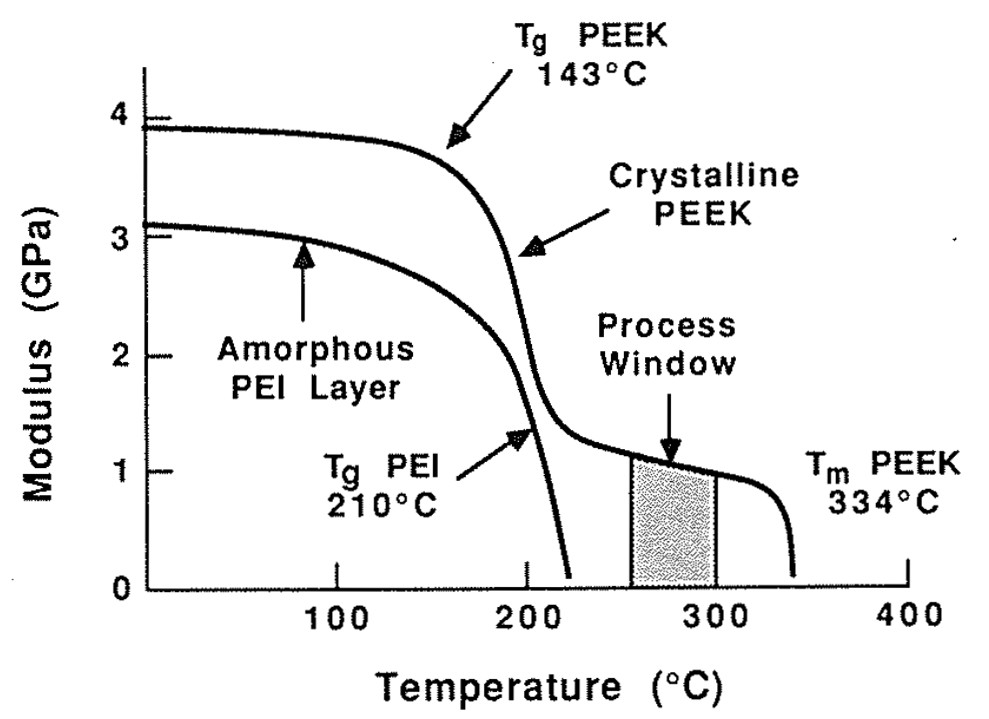
\includegraphics[width=0.55\textwidth]{Thermabond_Bastien1991.jpg}
	\caption{Modules du PEEK et du PEI illustrant la plage de température du procédé de soudage avec un film amorphe (tiré de \cite{Bastien1991}, reproduction avec autorisation)}
	\label{fig:thermabond_process}
\end{figure}

\FloatBarrier
Une seconde famille regroupe les procédés produisant un chauffage par friction, vibration ou ultrasons \cite{Bates2007d}. 
À l'aide d'un mouvement alternatif rapide, la friction entre les composants produit un échauffement local. 
Ce même effet peut également être obtenu à l'aide d'ultrasons en raison de l'hystérésis thermomécanique des matériaux. 
Ces méthodes pour joindre des composants sont rapides, mais peuvent induire un déplacement des fibres. 
Également, malgré ses très bonnes performances mécaniques \cite{Villegas2016}, l'application du soudage par ultrasons peut être complexe pour les jonctions sur de longues distances lorsqu'une approche point par point est utilisée en raison de l'interaction entre les soudures successives \cite{Zhao2018}. 
Cependant, en modifiant l'outillage et en le déplaçant progressivement le long de la soudure, il est possible de produire des joints continus \cite{Engelschall2019}.
Une autre famille de procédés regroupe les méthodes où le processus de soudage se produit en deux étapes distinctes. 
Dans un premier temps, les faces à joindre sont chauffées à l'aide de plaques chauffantes, de laser, d'infrarouges ou encore de gaz chaud \cite{Yousefpour2004a,Johnson1989}. 
En second lieu, les faces sont mises en contact pour obtenir la jonction. 
On peut également regrouper en une catégorie les procédés utilisant une source de chaleur électromagnétique. 
Dans cette famille, on retrouve le soudage par induction \cite{Rudolf2000a,Ahmed2006a,Farahani2018}, le soudage  par pertes diélectriques et par micro-ondes \cite{Wu2012,Bowler2006a,Menendez2010d}, et le soudage par résistance \cite{houghton1984bonding,Eveno1988,Taylor1991,McKnight1997}. 
Les procédés de chauffe par induction, pertes diélectriques ou micro-ondes sont basés sur l'utilisation d'un champ électromagnétique alternatif. 
La différence entre ces procédés réside dans la fréquence du champ employé, allant des centaines de \si{\kilo\hertz} en induction jusqu'au \si{\giga\hertz} pour le chauffage par micro-ondes. 
Finalement, le soudage par résistance utilise les pertes par résistance dans un conducteur électrique pour obtenir un chauffage local à l'aide de l'effet de Joule. 
Il s'agit d'une méthode rapide, répétable et pouvant être aisément mise à l'échelle pour produire de plus grandes soudures. 
Le reste des travaux présentés dans cette thèse porteront sur le soudage par résistance. 

\begin{figure}[h]
	\centering
	\usetikzlibrary{arrows,shapes,positioning,shadows,trees}
\usetikzlibrary{decorations.pathmorphing} % Pour obtenir des lignes de coupes aléatoires
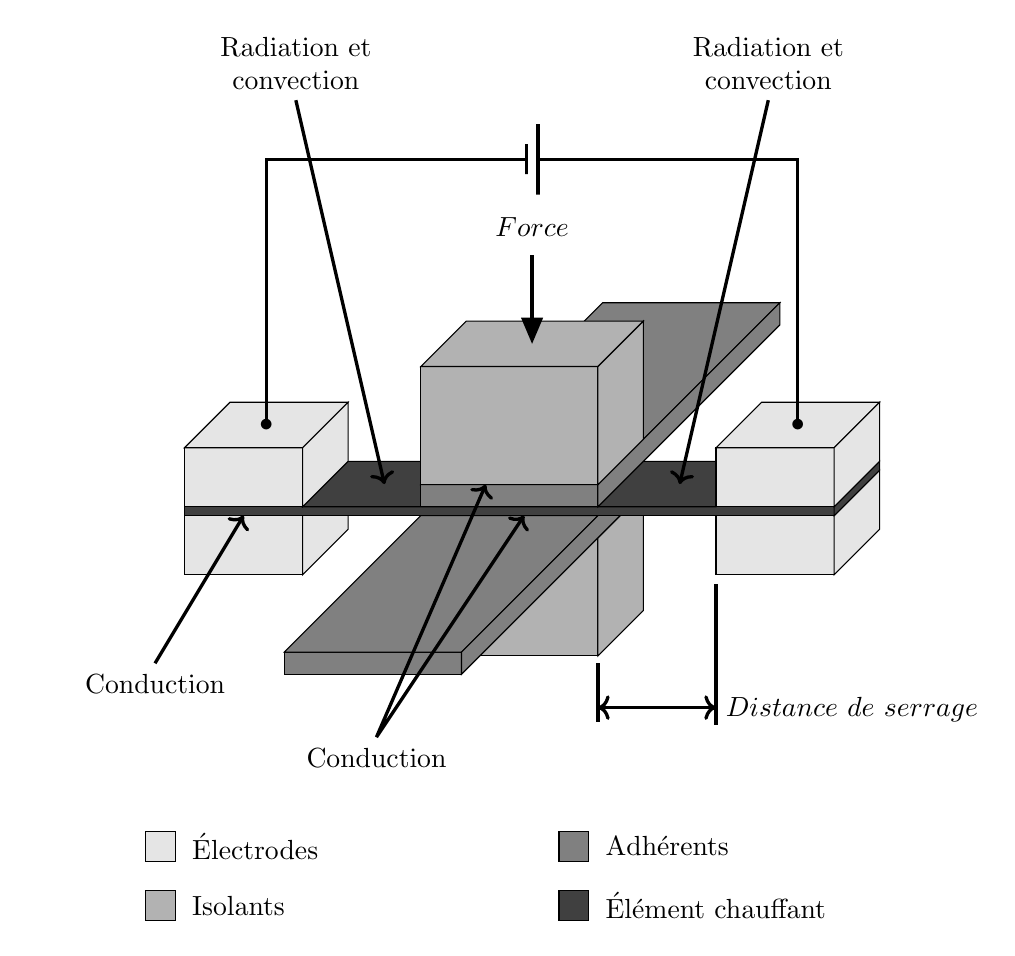
\begin{tikzpicture}[scale=0.75]


%Dimentions du bloc de connection
\def \largconnection{2}
\def \profconnection{2}
\def \hconnection{1.}

%Distance entre les deux blocs
\def \distance_connection{9}

%Épaisseur de l'élément résistif
\def \tele{0.15}

%Distance entre les blocs de connection et l'isolant
\def \gap{2}

%Dimensions des adhérent
\def \lcomp{6}
\def \tcomp{0.375}

%Épaisseur de l'isolant
\def \tbloc{2}

%Position et taille des annotations
\def \hsource{1.25*\profconnection}
\def \hpression{0.75*\profconnection}
\def \legende{0.5}
\def \distcotation{0.125}

%Couleurs
\def \colinsulator{blue!50}
\def \coladherend{green!50}
\def \colconnector{orange!60}
\def \colresistive{gray!50}

\def \colinsulator{black!30}
\def \coladherend{black!50}
\def \colconnector{black!10}
\def \colresistive{black!75}

%Bloc de pression inferieur
\draw[black,fill=\colinsulator] (\largconnection+\gap,-\tcomp-\tele-\tbloc,0) -- ++(0,\tbloc,0) -- ++(\distance_connection-\gap-\gap-\largconnection,0,0) -- ++(0,-\tbloc,0) -- cycle; %Face du devant
\draw[black,fill=\colinsulator] (\distance_connection-\gap,-\tcomp-\tele-\tbloc,0) -- ++(0,\tbloc,0) -- ++(0,0,-\profconnection) -- ++(0,-\tbloc,0) -- cycle; %Face de droite

%Adherant inferieur
\draw[black,fill=\coladherend] (\largconnection+\gap,-\tele-\tcomp,\lcomp) -- ++(0,\tcomp,0) -- ++(\distance_connection-\gap-\gap-\largconnection,0,0) -- ++(0,-\tcomp,0) -- cycle; %Face du devant
\draw[black,fill=\coladherend] (\largconnection+\gap,-\tele,\lcomp) -- ++(0,0,-\lcomp) -- ++(\distance_connection-\gap-\gap-\largconnection,0,0) -- ++(0,0,\lcomp) -- cycle; %Face du dessus
\draw[black,fill=\coladherend] (\distance_connection-\gap,-\tele,\lcomp) -- ++(0,-\tcomp,0) -- ++(0,0,-\lcomp-\profconnection) -- ++(0,\tcomp,0) -- cycle; %Face de droite

%Connection gauche inferieur
\draw[black, fill=\colconnector] (0,-\tele-\hconnection,0)--++(\largconnection,0,0)--++(0,\hconnection,0)--++(-\largconnection,0,0)--cycle; %Face du devant
\draw[black, fill=\colconnector] (\largconnection,-\tele-\hconnection,0)--++(0,\hconnection,0)-- ++(0,0,-\profconnection)--++(0,-\hconnection,0)--cycle; %Face de droite

%Connection droite inferieur
\draw[black, fill=\colconnector] (\distance_connection,-\tele-\hconnection,0)--++(\largconnection,0,0)--++(0,\hconnection,0)--++(-\largconnection,0,0)--cycle; %Face du devant
\draw[black, fill=\colconnector] (\largconnection+\distance_connection,-\tele-\hconnection,0)--++(0,\hconnection,0)--++(0,0,-\profconnection)--++(0,-\hconnection,0)--cycle; %Face de droite

%Element chauffant
\draw[black,fill=\colresistive] (0,0,0) -- (\largconnection+\distance_connection,0,0) -- ++(0,-\tele,0) -- (0,-\tele,0) -- cycle; %Face du devant
\draw[black,fill=\colresistive] (\largconnection,0,0) -- ++(0,0,-\profconnection) -- (\distance_connection,0,-\profconnection) -- (\distance_connection,0,0) -- cycle; %Face du dessus
\draw[black,fill=\colresistive] (\distance_connection+\largconnection,0,0) -- ++(0,0,-\profconnection) -- ++(0,-\tele,0) -- ++(0,0,\profconnection) -- cycle; %Face de droite

%Adherant superieur
\draw[black,fill=\coladherend] (\largconnection+\gap,0,0) -- ++(0,\tcomp,0) -- ++(\distance_connection-\gap-\gap-\largconnection,0,0) -- ++(0,-\tcomp,0) -- cycle; %Face du devant
\draw[black,fill=\coladherend] (\largconnection+\gap,\tcomp,0) -- ++(0,0,-\lcomp-\profconnection) -- ++(\distance_connection-\gap-\gap-\largconnection,0,0) -- ++(0,0,\lcomp+\profconnection) -- cycle; %Face du dessus
\draw[black,fill=\coladherend] (\distance_connection-\gap,\tcomp,0) -- ++(0,-\tcomp,0) -- ++(0,0,-\lcomp-\profconnection) -- ++(0,\tcomp,0) -- cycle; %Face de droite

%Connection gauche superieure
\draw[black, fill=\colconnector] (0,0,0)--(\largconnection,0,0)--++(0,\hconnection,0)--(0,\hconnection,0)--cycle; %Face du devant
\draw[black, fill=\colconnector] (0,\hconnection,0)--++(\largconnection,0,0)--++(0,0,-\profconnection)--++(-\largconnection,0,0)--cycle; %Face du dessus
\draw[black, fill=\colconnector] (\largconnection,0,0)--++(0,\hconnection,0)-- ++(0,0,-\profconnection)--++(0,-\hconnection,0)--cycle; %Face de droite

%Connection droite superieure
\draw[black, fill=\colconnector] (\distance_connection,0,0)--++(\largconnection,0,0)--++(0,\hconnection,0)--++(-\largconnection,0,0)--cycle; %Face du devant
\draw[black, fill=\colconnector] (\distance_connection,\hconnection,0)--++(\largconnection,0,0)--++(0,0,-\profconnection)--++(-\largconnection,0,-0)--cycle; %Face du dessus
\draw[black, fill=\colconnector] (\largconnection+\distance_connection,0,0)--++(0,\hconnection,0)--++(0,0,-\profconnection)--++(0,-\hconnection,0)--cycle; %Face de droite

%Bloc de pression superieur
\draw[black,fill=\colinsulator] (\largconnection+\gap,\tcomp,0) -- ++(0,\tbloc,0) -- ++(\distance_connection-\gap-\gap-\largconnection,0,0) -- ++(0,-\tbloc,0) -- cycle; %Face du devant
\draw[black,fill=\colinsulator] (\largconnection+\gap,\tcomp+\tbloc,0) -- ++(0,0,-\profconnection) -- ++(\distance_connection-\gap-\gap-\largconnection,0,0) -- ++(0,0,\profconnection) -- cycle; %Face du dessus
\draw[black,fill=\colinsulator] (\distance_connection-\gap,\tcomp,0) -- ++(0,\tbloc,0) -- ++(0,0,-\profconnection) -- ++(0,-\tbloc,0) -- cycle; %Face de droite

%Connection de la source de puissance
\draw [very thick] (0.5*\largconnection,\hconnection,-0.5*\profconnection) -- ++(0,\hsource+\tbloc,0) -- ++(0.5*\distance_connection-0.1,0,0) -- ++(0,-0.25,0) -- ++(0,0.5,0);
\draw [very thick] (0.5*\largconnection+\distance_connection,\hconnection,-0.5*\profconnection) -- ++(0,\hsource+\tbloc,0) -- ++ (-0.5*\distance_connection+0.1,0,0) -- ++(0,-0.6,0) -- ++ (0,1.2,0);
\draw (0.5*\largconnection,\hconnection,-0.5*\profconnection) node {$\bullet$} ;
\draw (0.5*\largconnection+\distance_connection,\hconnection,-0.5*\profconnection) node {$\bullet$} ;

%Pression
\draw [very thick, -triangle 45] (0.5*\largconnection+0.5*\distance_connection,\tbloc+\tcomp+\hpression,-0.5*\profconnection) -> ++(0,-\hpression,0);
\draw (0.5*\largconnection+0.5*\distance_connection,\tbloc+\tcomp+\hpression+0.15,-0.5*\profconnection) node[above] {$Force$};

%Clamping distance
\draw [very thick, black] (\distance_connection-\gap,-\tcomp-\tele-\tbloc-\distcotation,0) -- ++(0,-1,0);
\draw [very thick, black] (\distance_connection,-0.5*\tcomp-\hconnection-\distcotation,0) -- ++(0,-1-\tbloc+\hconnection-\tcomp,0);
\draw [very thick, black, <->] ((\distance_connection-\gap,-\tcomp-\tele-\tbloc-\distcotation-0.75,0) -- ++ (\gap,0,0);
\draw (\distance_connection,-0.5*\tcomp-\tcomp-\distcotation-\tbloc-.75,0) node[right] {$Distance \ de \ serrage$};

%Identification des modes de refroidissement
\draw [very thick,<-] (\largconnection+0.5*\gap,0,-0.5*\profconnection) -- ++(-1.5,6.5,0) node[above, text width=3cm, align=center] {{Radiation et \\ convection}};
\draw [very thick,<-]  (\distance_connection-0.5*\gap,0,-0.5*\profconnection) -- ++(1.5,6.5,0) node[above, text width=3cm, align=center] {{Radiation et \\ convection}};
\draw [very thick,<-]  (0.5*\largconnection,-\tele,0) -- ++(-1.5,-2.5,0) node[below, text width=3cm, align=center] {{Conduction}};
\draw [very thick,<->]  (0.5*\distance_connection+0.625*\gap,-\tele,0) -- ++(-2.5,-3.75,0) node[below, text width=3cm, align=center] {{Conduction}} --(0.5*\distance_connection+0.3*\gap,\tcomp,0) ;


%Legende
\begin{scope}[yshift=-11.cm, xshift=-5.5cm]

	\begin{scope}[xshift=-7cm]
		\draw [black, fill=\colconnector] (\distance_connection+1.42*\profconnection,2.5*\tbloc) rectangle ++(\legende,\legende);
		\draw (\distance_connection+1.42*\profconnection+1.25*\legende,2.5*\tbloc+0.5*\legende) node[right]{Électrodes} ;

		\draw [black, fill=\colinsulator] (\distance_connection+1.42*\profconnection,2.5*\tbloc-2*\legende) rectangle ++(\legende,\legende);
		\draw (\distance_connection+1.42*\profconnection+1.25*\legende,2.5*\tbloc-1.5*\legende) node[right]{Isolants} ;
	\end{scope}

	\draw [black, fill=\coladherend] (\distance_connection+1.42*\profconnection,2.5*\tbloc) rectangle ++(\legende,\legende);
	\draw (\distance_connection+1.42*\profconnection+1.25*\legende,2.5*\tbloc+0.5*\legende) node[right]{Adhérents} ;

	\draw [black, fill=\colresistive] (\distance_connection+1.42*\profconnection,2.5*\tbloc-2*\legende) rectangle ++(\legende,\legende);
	\draw (\distance_connection+1.42*\profconnection+1.25*\legende,2.5*\tbloc-1.5*\legende) node[right]{Élément chauffant} ;
\end{scope}
\end{tikzpicture}

	\caption{Schéma du procédé de soudage par résistance avec identification des modes de conduction de chaleur}
	\label{fig:schema_soudage_resistance}
\end{figure}

Lors du soudage par résistance, un élément chauffant poreux est positionné entre les adhérents (Fig. \ref{fig:schema_soudage_resistance}). 
Généralement, des blocs isolants sont positionnés autour de la soudure pour réduire les pertes thermiques. 
Des électrodes sont fixées aux deux extrémités de l'élément chauffant à une distance variable du bord des adhérents, nommée «distance de serrage». 
Avant d'appliquer un courant dans le système et tout au long du procédé de soudage, une force est appliquée sur la zone à souder. 
Après un temps prédéterminé, la source électrique est arrêtée tout en maintenant la pression sur la soudure pendant le refroidissement. 
Une fois la soudure refroidie en dessous de la température de transition vitreuse des polymères, il est possible de retirer du montage l'assemblage obtenu. 
Il est à noter que l'élément chauffant reste captif de la soudure à la fin du procédé. 
La possibilité de produire des soudures continues en soudage par résistance a également été démontrée en laboratoire \cite{Shi2015a}. 
Les équations de contact intime et d'autohésion par diffusion des chaînes en situation de soudage non isotherme ont été appliquées par Ageorges \cite{Ageorges1998} et Colak \cite{Colak2002} afin d'approximer théoriquement des fenêtres d'opération. 

Si on fixe la géométrie du montage de soudage et le choix des matériaux, les principaux paramètres ayant une influence sur la qualité du joint sont 
\begin{inparaenum}[(1)]
	\item la puissance électrique, 
	\item le temps de soudage, 
	\item les effets de bords et les modes de conduction de chaleur, et
	\item la pression appliquée sur la soudure. 
\end{inparaenum}
Globalement, il faut également tenir compte des propriétés des matériaux employés ainsi que de la géométrie des composants du montage. 

\begin{figure}[h]
	\centering
	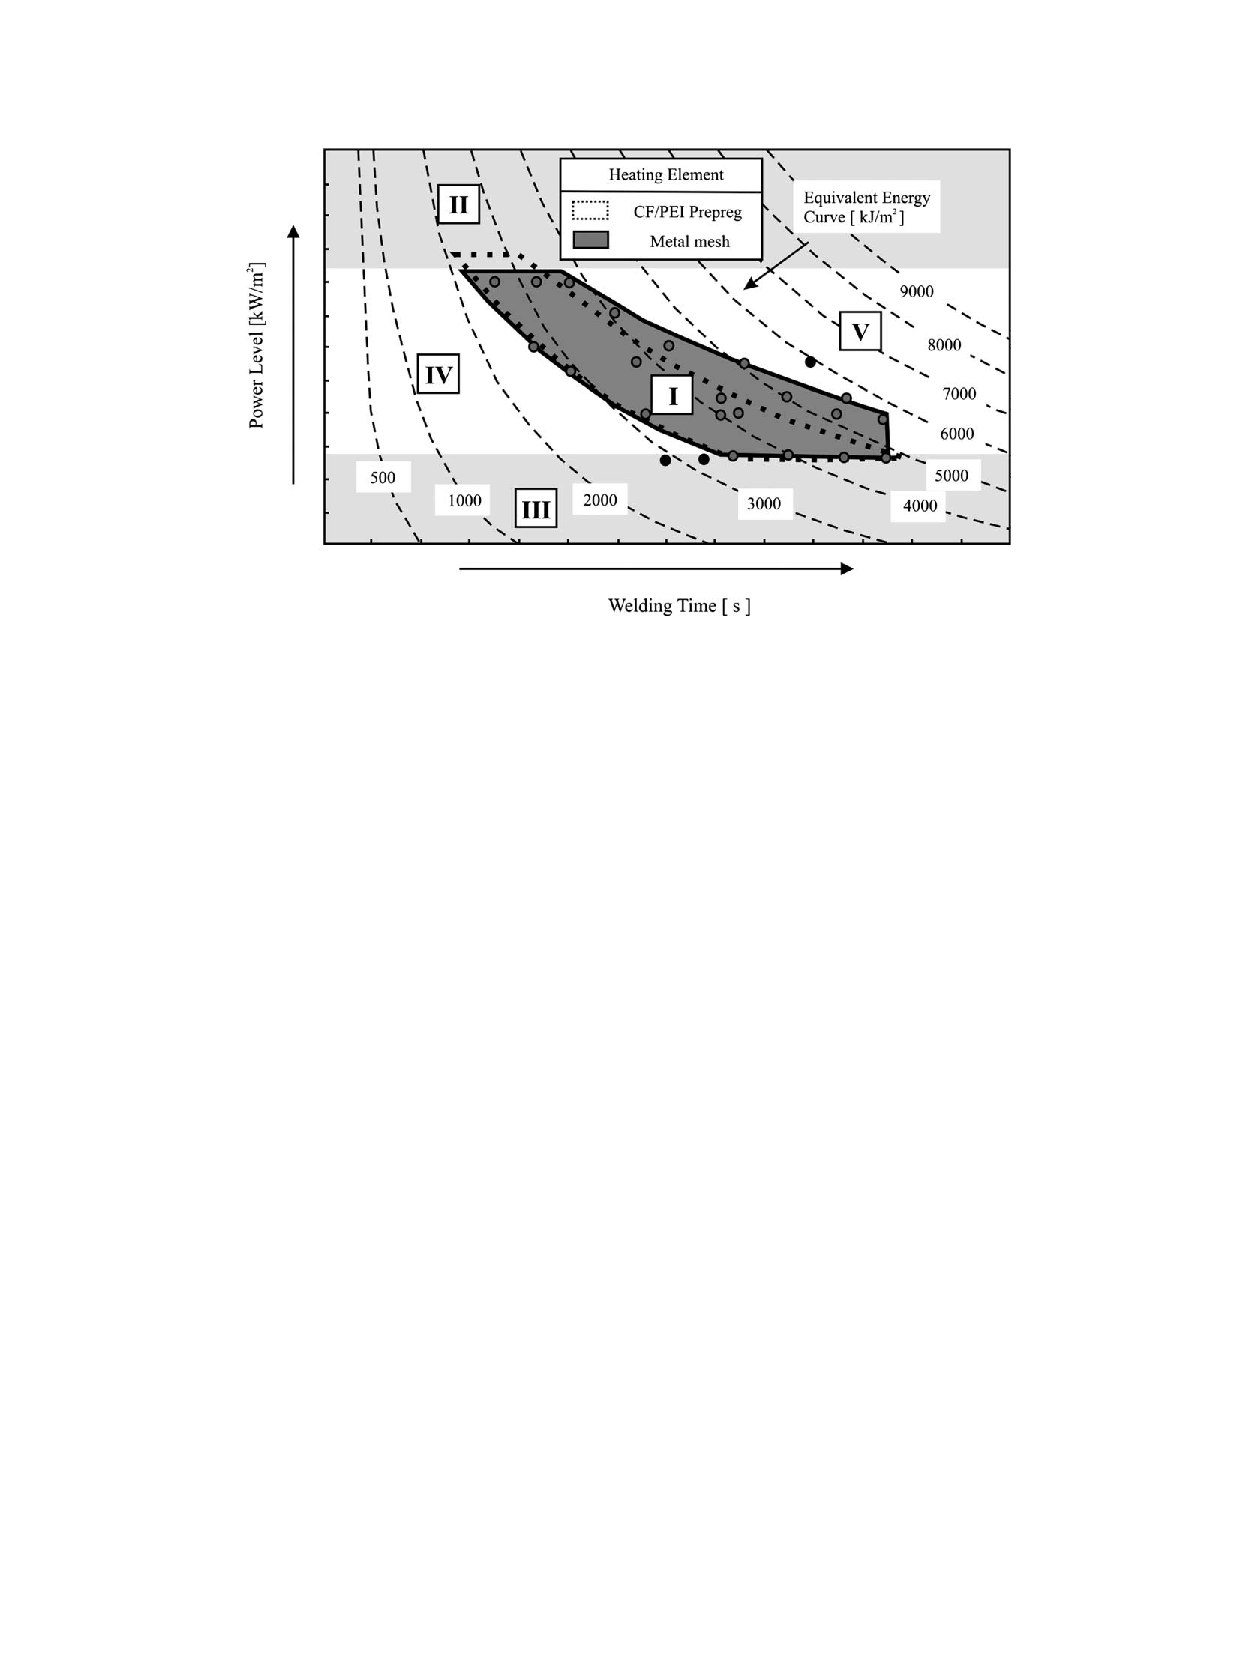
\includegraphics[scale=0.85]{process_window}
	\caption{Fenêtre de puissance pour le procédé de soudage (tirée de \cite{Stavrov2005a}, reproduction avec autorisation)}
	\label{fig:process_window}
\end{figure}

\FloatBarrier
Afin d'optimiser la qualité de la soudure, la puissance électrique et le temps de soudage peuvent facilement être modifiés. 
La plage de puissance ainsi que l'énergie nécessaire (produit de la puissance et du temps) à la production d'une soudure satisfaisante sont documentées dans la littérature \cite{Hou1999a}. 
Lors de l'utilisation de grillages en acier inoxydable comme éléments chauffants, des puissances surfaciques allant de 80 à \SI[locale=FR]{150}{\kilo\watt\per\square\metre} permettent typiquement de produire des soudures satisfaisantes. 
D'autres auteurs (tels que Dubé) ont également utilisé des puissances allant jusqu'à \SI[locale=FR]{282}{\kilo\watt\per\square\metre} \cite{Dube2007} avec des temps plus courts. 
Certains auteurs (tels que Arias) utilisent également de très fortes puissances pulsées de l'ordre de \SI[locale=FR]{600}{\kilo\watt\per\square\metre} avec un temps de repos de quelques secondes entre chaque pulsation afin d'obtenir une température plus uniforme dans la zone soudée et de réduire la quantité d'énergie requise  \cite{Arias1996}. 
Dans presque tous ces cas, les auteurs ont appliqué le courant en maintenant une tension constante ou en produisant une rampe de voltage. 
La résistance des éléments chauffants en acier inoxydable augmente lors de la chauffe entraînant une réduction de la puissance dissipée dans le joint à plus haute température. 
La figure \ref{fig:process_window} présente une fenêtre de puissance de soudage en fonction du temps afin d'obtenir un soudage entre des pièces en composites avec un élément chauffant en acier inoxydable ou en composite de fibre de carbone avec une matrice en PEI. 
Ce graphique présente également des courbes d'énergie équivalente. 
On peut obtenir l'énergie produite en multipliant la puissance au temps d'application selon l'équation : 

\begin{equation}
E = P \times t
\end{equation}

où $E$ est la quantité d'énergie en Joules, $P$ est la puissance en Watts et $t$ est le temps en secondes. 
On peut obtenir la puissance d'un élément chauffant de section constante, en fonction de ses propriétés électriques et de ses dimensions, à l'aide des équations suivantes. Dans ces équations, $V$ est la tension en volts, $I$ est l'intensité du courant en ampères, $R$ est la résistance en $\ohm$, $L$ est la longueur en mètres du conducteur, $A_s$ est l'aire de la section du conducteur en mètres carrés et $\rho_{ele}$ est la résistivité en $\ohm \cdot$mètres. 

\begin{equation}
P = V \times I
\end{equation}

\begin{equation}
P = R \times I^2
\end{equation}

\begin{equation}
P = \frac{\rho_{ele} \times L}{A_s} \ I^2
\end{equation}

\begin{equation}
P = \frac{V^2}{\rho_{ele}} \ \frac{A_s}{L}
\end{equation}

Il est possible de lier la résistivité ($\rho_{ele}$) d'un matériau à sa conductivité ($\sigma$) en Siemens par mètres à l'aide de l'équation suivante :

\begin{equation}
\sigma = \frac{1}{\rho_{ele}}
\end{equation}

Dans le cas des éléments pour le soudage résistif, ces équations sont simplifiées sous la forme suivante où $l$ est la largeur en mètre du grillage et $\gamma$ est la résistivité spécifique en $\ohm$ :

\begin{equation}
R = \gamma \ \frac{L}{l}
\label{EQ:resistance_element_chauffant}
\end{equation}

Pour utiliser l'équation \ref{EQ:resistance_element_chauffant}, il est nécessaire de caractériser au préalable l'élément chauffant afin de connaître sa résistance spécifique. 
Cette dernière équation pose également l'hypothèse d'un élément de composition relativement homogène. 
Les effets des dimensions des mailles ainsi que le diamètre des fils ont été étudiés dans la littérature et il a été trouvé que le ratio entre le ratio d'aire ouverte et le diamètre du fil est un critère important pour le soudage avec un grillage métallique \cite{Dube2012a}. 

Pour ce qui est des effets de bords et des modes de conduction de chaleur, cet effet est principalement dépendant de la géométrie du montage et de la nature des matériaux. 
Cependant, pour un montage de soudage donné, un contrôle limité de ce paramètre est parfois possible en modifiant la distance de serrage des électrodes. 
Comme indiqué à la figure \ref{fig:schema_soudage_resistance}, les pertes thermiques de l'élément chauffant changent de mode de diffusion en fonction de leur position dans la soudure. 
Dans les zones où l'élément chauffant est positionné entre les adhérents composites ou lorsqu'il est en contact avec les électrodes, la diffusion thermique se produit principalement par conduction. 
Dans les zones où l'élément chauffant est exposé (entre les bords des adhérents et les électrodes), les pertes thermiques se produisent plutôt par radiation et convection naturelle. 
Puisque ces derniers modes de transfert de chaleur sont moins efficaces, un certain contrôle de la température au bord du laminé est possible en ajustant la distance de serrage \cite{Talbot2013}. 
Il est impossible d'éliminer totalement ces effets de bord, mais il est possible de viser des paramètres de soudage qui en réduisent l'effet. 

En ce qui concerne la pression appliquée sur la soudure, plusieurs chercheurs ont présenté l'effet de la pression sur la qualité des soudures obtenues. 
En premier lieu, pour les soudures de laminés avec une matrice en PEI, Ageorges \cite{Ageorges2000a} a observé des signes de déconsolidation des laminés lorsqu'une faible pression, de l'ordre de \SI[locale=FR]{0.1}{\mega\pascal}, est employée.
Il a aussi noté le déplacement des fibres et un trop grand écoulement causé par la compression du laminé lorsqu'une pression supérieure à \SI[locale=FR]{1.6}{\mega\pascal} est employée. 
Il définit au final une plage entre 0,2 et \SI[locale=FR]{1.6}{\mega\pascal} comme cible. 
Une autre étude plus détaillée \cite{Shi2017} a observé l'effet de la pression sur la formation de porosités et la déconsolidation pour des laminés de fibres de verre et PEI. 
Les résultats ont démontré qu'une pression d'au moins \SI[locale=FR]{0.8}{\mega\pascal} est nécessaire pour éliminer les porosités à l'interface causées par l'humidité et la déconsolidation du laminé. 

\begin{figure}[h]
	\centering
	\usetikzlibrary{arrows,shapes,positioning,shadows,trees,arrows.meta}
\usetikzlibrary{decorations.pathmorphing} % Pour obtenir des lignes de coupes aléatoires
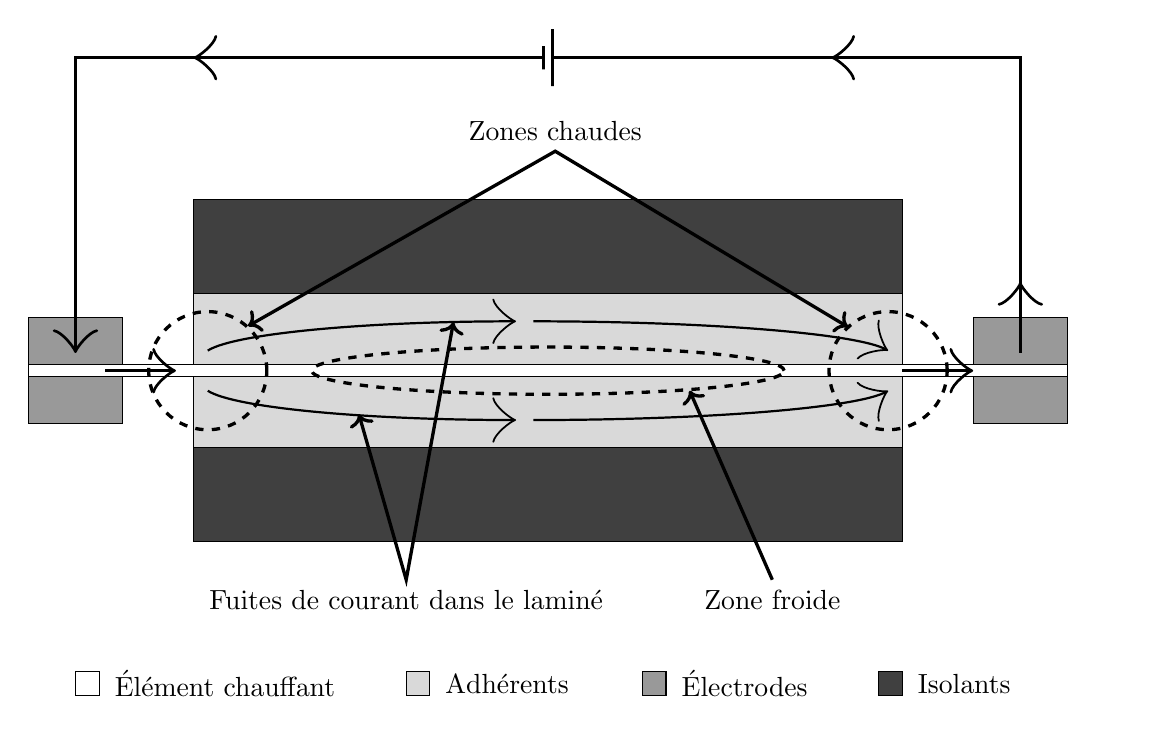
\begin{tikzpicture}[scale=0.6]


%Dimentions du bloc de connection
\def \largconnection{2}
\def \hconnection{1.}

%Distance entre les deux blocs
\def \distance_connection{20}

%Épaisseur de l'élément résistif
\def \tele{0.25}

%Distance entre les blocs de connection et l'isolant
\def \gap{1.5}

%Dimensions des adhérent
\def \tcomp{1.5}

%Épaisseur de l'isolant
\def \tbloc{2}

%Position et taille des annotations
\def \hsource{3.5}
\def \legende{0.5}
\def \distcotation{0.125}

%Couleurs
\def \colinsulator{blue!50}
\def \coladherend{green!50}
\def \colconnector{orange!60}
\def \colresistive{gray!50}

\def \colinsulator{black!75}
\def \coladherend{black!15}
\def \colconnector{black!40}
\def \colresistive{black!0}

%Bloc de pression inferieur
\draw[black,fill=\colinsulator] (\largconnection+\gap,-\tcomp-\tele-\tbloc) -- ++(0,\tbloc) -- ++(\distance_connection-\gap-\gap-\largconnection,0) -- ++(0,-\tbloc) -- cycle; %Face du devant

%Adherant inferieur
\draw[black,fill=\coladherend] (\largconnection+\gap,-\tele-\tcomp) -- ++(0,\tcomp) -- ++(\distance_connection-\gap-\gap-\largconnection,0) -- ++(0,-\tcomp) -- cycle; %Face du devant

%Connection gauche inferieur
\draw[black, fill=\colconnector] (0,-\tele-\hconnection)--++(\largconnection,0)--++(0,\hconnection)--++(-\largconnection,0)--cycle; %Face du devant


%Connection droite inferieur
\draw[black, fill=\colconnector] (\distance_connection,-\tele-\hconnection,0)--++(\largconnection,0,0)--++(0,\hconnection,0)--++(-\largconnection,0,0)--cycle; %Face du devant


%Element chauffant
\draw[black,fill=\colresistive] (0,0,0) -- (\largconnection+\distance_connection,0,0) -- ++(0,-\tele,0) -- (0,-\tele,0) -- cycle; %Face du devant


%Adherant superieur
\draw[black,fill=\coladherend] (\largconnection+\gap,0,0) -- ++(0,\tcomp,0) -- ++(\distance_connection-\gap-\gap-\largconnection,0,0) -- ++(0,-\tcomp,0) -- cycle; %Face du devant


%Connection gauche superieure
\draw[black, fill=\colconnector] (0,0,0)--(\largconnection,0,0)--++(0,\hconnection,0)--(0,\hconnection,0)--cycle; %Face du devant

%Connection droite superieure
\draw[black, fill=\colconnector] (\distance_connection,0,0)--++(\largconnection,0,0)--++(0,\hconnection,0)--++(-\largconnection,0,0)--cycle; %Face du devant

%Bloc de pression superieur
\draw[black,fill=\colinsulator] (\largconnection+\gap,\tcomp,0) -- ++(0,\tbloc,0) -- ++(\distance_connection-\gap-\gap-\largconnection,0,0) -- ++(0,-\tbloc,0) -- cycle; %Face du devant


%Connection de la source de puissance
\draw [very thick] (0.5*\largconnection,\hconnection) -- ++(0,\hsource+\tbloc) -- ++(0.5*\distance_connection-0.1,0) -- ++(0,-0.25) -- ++(0,0.5);
\draw [very thick] (0.5*\largconnection+\distance_connection,\hconnection) -- ++(0,\hsource+\tbloc) -- ++ (-0.5*\distance_connection+0.1,0) -- ++(0,-0.6) -- ++ (0,1.2);


%Courant dans le laminé
\draw[thick, -{Classical TikZ Rightarrow[length=3mm]} ] (\largconnection+1.2*\gap,0.2*\tcomp) arc (170 : 90 : {0.5*\distance_connection-2.25*\gap} and 0.75);
\draw[thick, -{Classical TikZ Rightarrow[length=3mm]} ] (\largconnection+1.2*\gap,-0.2*\tcomp-\tele) arc (-10 : -90 : -{0.5*\distance_connection+2.25*\gap} and 0.75);
\draw [thick, {Classical TikZ Rightarrow[length=3mm]}- ] (\distance_connection-1.2*\gap,0.2*\tcomp) arc (10 : 90 : {0.25*\distance_connection+1.75*\gap} and 0.75);
\draw [thick, {Classical TikZ Rightarrow[length=3mm]}- ] (\distance_connection-1.2*\gap,-0.2*\tcomp-\tele) arc (-10 : -90 : {0.25*\distance_connection+1.75*\gap} and 0.75);
\draw [very thick, {Classical TikZ Rightarrow[length=3mm]}- ] (0.5*\largconnection,0.25*\hconnection) -- ++(0,1.5);
\draw [very thick, -{Classical TikZ Rightarrow[length=3mm]}] (0.5*\largconnection+\distance_connection,0.25*\hconnection) -- ++(0,1.5);
\draw [very thick, -{Classical TikZ Rightarrow[length=3mm]}] (\largconnection-0.25*\gap,-0.5*\tele) -- ++(1*\gap,0);
\draw [very thick, -{Classical TikZ Rightarrow[length=3mm]}] (\distance_connection-1*\gap,-0.5*\tele) -- ++(1.*\gap,0);
\draw [very thick, -{Classical TikZ Rightarrow[length=3mm]}] (\distance_connection-1*\gap,\hconnection+\hsource+\tbloc) -- ++(-\gap,0);
\draw [very thick, -{Classical TikZ Rightarrow[length=3mm]}] (\largconnection+2*\gap,\hconnection+\hsource+\tbloc) -- ++(-1.*\gap,0);

%Identification des fuites de courant
\draw [very thick,<->]  (0.35*\distance_connection,-\tele-0.8) -- ++(1,-3.5) node[below, text width=9cm, align=center] {{Fuites de courant dans le laminé}} --(0.45*\distance_connection,\tcomp-0.6) ;

% zones chaudes
\begin{scope}[radius=1.25, very thick, dashed]
\draw (\largconnection+\gap+0.3,-0.5*\tele) circle ;
\draw (-\gap+\distance_connection-0.3,-0.5*\tele) circle ;
\end{scope}
\draw [very thick,<->]  (\largconnection+\gap+1.155,0.82) -- ++(6.5,3.7) node[above, text width=9cm, align=center] {{Zones chaudes}} --(-\gap+\distance_connection-1.15,\tcomp-0.7) ;

% zone froide
\draw [very thick, dashed] (0.5*\distance_connection+0.5*\largconnection,-0.5*\tele) ellipse [x radius=5,y radius=0.5] ;
\draw [very thick,<-]  (0.7*\distance_connection,-\tele-0.3) -- ++(1.75,-4) node[below, text width=9cm, align=center] {{Zone froide}} ;

%Legende
\begin{scope}[yshift=-12.cm, xshift=1cm]

\begin{scope}[xshift=12cm]
\draw [black, fill=\colconnector] (0,2.5*\tbloc) rectangle ++(\legende,\legende);
\draw (1.25*\legende,2.5*\tbloc+0.5*\legende) node[right]{Électrodes} ;
\end{scope}

\begin{scope}[xshift=7cm]
\draw [black, fill=\coladherend] (0,2.5*\tbloc) rectangle ++(\legende,\legende);
\draw (1.25*\legende,2.5*\tbloc+0.5*\legende) node[right]{Adhérents} ;
\end{scope}

\begin{scope}[xshift=0cm]
\draw [black, fill=\colresistive] (0,2.5*\tbloc) rectangle ++(\legende,\legende);
\draw (1.25*\legende,2.5*\tbloc+0.5*\legende) node[right]{Élément chauffant} ;
\end{scope}

\begin{scope}[xshift=17cm]
\draw [black, fill=\colinsulator] (0,2.5*\tbloc) rectangle ++(\legende,\legende);
\draw (1.25*\legende,2.5*\tbloc+0.5*\legende) node[right]{Isolants} ;
\end{scope}

\end{scope}
\end{tikzpicture}

	\caption{Schéma du phénomène de fuite de courant}
	\label{fig:schema_fuite_de_courant}
\end{figure}

Un phénomène à surveiller lors du soudage résistif est la fuite de courant dans le corps des laminés de fibres de carbone. 
Ce phénomène peut se produire lorsque les bords de l'élément chauffant entrent en contact électrique avec les fibres de carbone du laminé et forment un circuit électrique parallèle à l'élément résistif \cite{Hou1999a,Ageorges2000}. 
Ce nouveau circuit réduit le chauffage de la zone soudée, peut empêcher la soudure au centre du joint et peut dégrader le polymère aux bords \cite{Dube2008}. 
On observe alors des zones chaudes aux bords des laminés et une zone froide au centre (Fig. \ref{fig:schema_fuite_de_courant}). 
Plusieurs approches existent pour éliminer ce problème. 
Il est possible d'ajouter une couche de fibre de verre isolante entre l'élément chauffant et le laminé \cite{Hou1999a}. 
Cette solution a le désavantage d'ajouter un élément étranger dans la zone soudée et d'augmenter l'épaisseur des joints. 
Il est également possible d'isoler le grillage métallique à l'aide d'un revêtement isolant \cite{Dube2008,Dube2009a}. 
Ce revêtement empêche tout contact électrique entre les fibres et l'élément chauffant. 
Finalement, il est également possible d'employer une couche d'un polymère possédant une température de mise en forme inférieure à la température de fonte du polymère de base \cite{Stavrov2005a}. 

Le soudage par résistances des composites thermoplastiques est généralement réalisé avec un élément chauffant en acier inoxydable ou encore en fibre de carbone. 
Initialement, il était naturel pour les chercheurs d'utiliser un élément chauffant en composites à fibre de carbone \cite{Ageorges2000a,houghton1984bonding,Eveno1988}. 
Cependant, des problèmes persistants étaient causés par la connexion électrique avec les fibres, le manque de répétabilité dans les résultats obtenus et la mise à l'échelle \cite{McKnight1997}. 
Le passage à des éléments chauffants en acier inoxydable a permis d'améliorer grandement la répétabilité du procédé ainsi que sa capacité à être mis à l'échelle \cite{Hou1999a}.  
Cependant, dans certaines circonstances, le manque d'adhésion entre les éléments chauffants en acier inoxydable et la matrice peut être le point faible d'une soudure par résistance \cite{Dube2007,Dube2012a,Dube2009a,Shi2014,Shi2015a}. 
Également, les éléments chauffants métalliques peuvent poser d'autres problèmes tels qu'une augmentation de l'écho radar \cite{Ageorges2001a}. 

\FloatBarrier
\subsection{Soudage avec matériaux mixtes}

Les composites à matrice thermoplastiques peuvent également être joints à d'autres matériaux. 
Plusieurs chercheurs travaillent au soudage entre des adhérents thermoplastiques et métalliques. 
Les méthodes employées varient du soudage au point par friction \cite{Goushegir2016}, au soudage par ultrasons \cite{Balle2009,Kruger2004} jusqu'à des combinaisons de soudage par laser avec un chauffage par induction \cite{Weidmann2018}. 
Ce dernier exemple est d'ailleurs intéressant par son approche où ils texturent d'abord l'adhérent métallique à l'aide d'un laser. 
Lors du soudage subséquent, le polymère vient remplir les porosités créées en surface pour obtenir un blocage mécanique entre les matériaux. 
Ce procédé a d'ailleurs fait l'objet d'une démonstration technologique visant à présenter une cellule de production automatisée pour des pièces du domaine automobile \cite{Gardiner2019a}. 

En plus des métaux, il est possible, dans certains cas de souder des adhérents en composites à matrice thermodurcissable. 
En employant une couche de polymère thermoplastique moulée avec le thermodurcissable lors de sa fabrication, des chercheurs ont pu souder des composites thermoplastiques avec des pièces en époxy \cite{Lionetto2018a,FernandezVillegas2015}.

\section{Nanocomposites conducteurs}

Les nanocomposites sont définis par l'Office québécois de la langue française depuis 2005 comme : 

\begin{quote}
	\textit{Matériau qui comporte deux ou plusieurs phases distinctes dont une au moins intègre des éléments qui possèdent une dimension pouvant varier entre 1 et 100 nanomètres.}
\end{quote}

Les nanocomposites sont constitués, au minimum, d'une matrice, souvent polymérique, et de particules de taille nanométriques. 
L'ajout de nanoparticules aux polymères permet entre autres de modifier leurs propriétés mécaniques \cite{Thostenson2002a}, électriques \cite{Zheng2003a}, optiques \cite{Hu2014} et thermiques \cite{Diez-Pascual2009, Al-Saleh2009c}. 
Les nanocomposites trouvent des applications dans plusieurs domaines comme, par exemple, la protection contre la foudre et les interférences électromagnétiques, le dégivrage des surfaces, les capteurs et la cryptographie \cite{Andrews2001, Thostenson2001c, Mittal2014h, Gaztelumendi2017, Chu2014, Hu2016, Al-Saleh2009, Chopra2003}. 

Les modifications des propriétés conférées par les nanoparticules sont dépendantes de leurs propriétés propres ainsi que de leur géométrie. 
Les propriétés exceptionnelles des nanoparticules proviennent en partie du ratio entre leur surface et leur volume. 
Elles exposent des surfaces spécifiques beaucoup plus importantes que tout autre matériau macroscopique. 

En raison de leur excellente conductivité électrique, les nanoparticules à base de carbone sont utilisées dans ce projet. 
Les nanoparticules métalliques telles que les nanofibres d'argent ou de cuivre n'ont pas été retenues au début du projet en raison de leur coût plus élevé et des faibles volumes disponibles commercialement. 
Pour cette raison, les prochaines sections de la revue de l'état des connaissances se concentrent sur les nanoparticules à base de carbone ainsi que sur leurs nanocomposites associés. 

\subsection{Nanotubes de carbone}

Découverts accidentellement en 1991 \cite{iijima1991}, les nanotubes de carbones se retrouvent maintenant dans presque tous les domaines de la science des matériaux et de nouvelles applications leur sont trouvées régulièrement. 
Les nanotubes de carbone sont composés d'une structure régulière de feuilles graphitiques de carbone enroulées et jointes pour former un ou des tubes concentriques qui peuvent être refermés aux extrémités par des structures sphériques (Fig. \ref{structure_nanotube}). 
Généralement, leur diamètre varie entre 2 et \SI{80}{\nano\metre} en fonction du nombre de couches et ils peuvent présenter des rapports de forme supérieurs à 1000. 

\begin{figure}[htb]
	\centering
	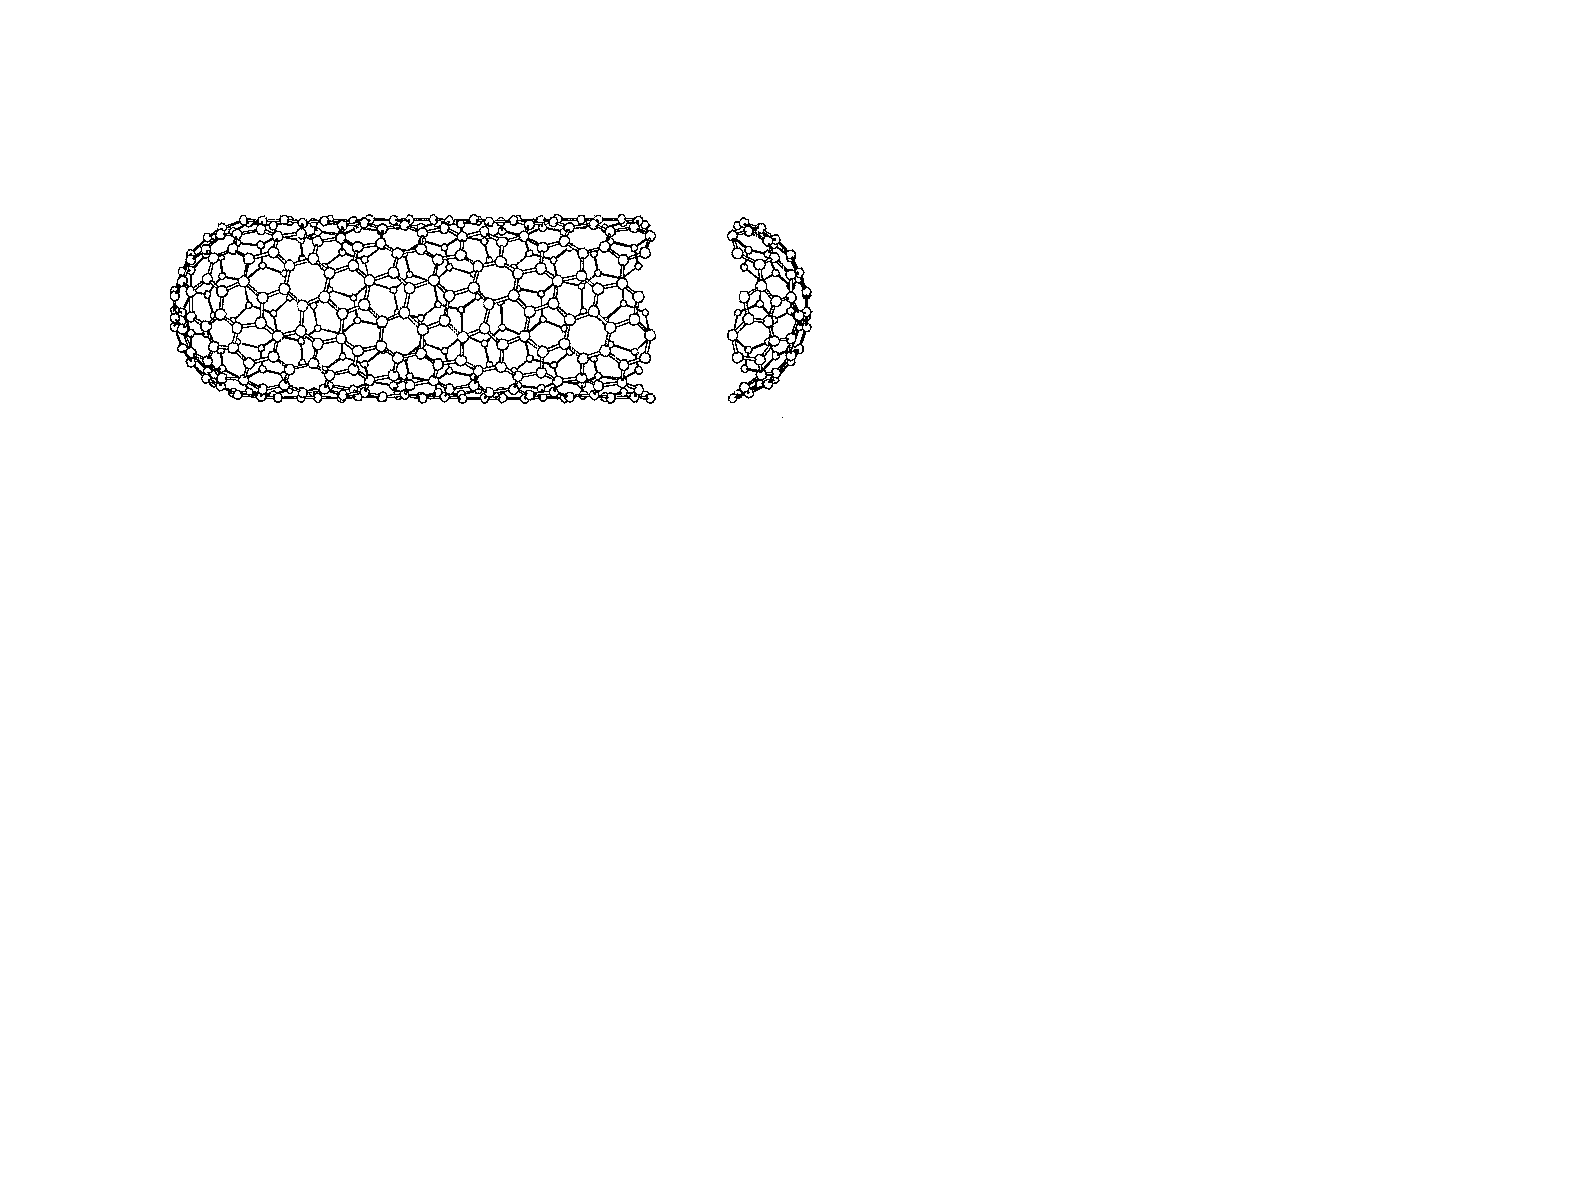
\includegraphics[width=0.5\textwidth]{Saito1992.pdf}
	\caption{Structure d'un nanotube de carbone (adapté de \cite{Saito1992}, reproduction avec autorisation)}
	\label{structure_nanotube}
\end{figure}

On différencie les nanotubes à simple paroi des nanotubes à parois multiples où plusieurs tubes se forment de façon concentrique. 
Le comportement des nanotubes est fonction de l'angle d'hélice de la structure. 
Pour les nanotubes à simple paroi on peut obtenir des nanotubes aux propriétés métalliques jusqu'à semi-conductrices avec des variations de cet angle \cite{Saito1992}. 
Des traitements permettent de purifier les nanotubes et surtout de les séparer selon leur comportement \cite{Makama2013}. 
Généralement, pour les nanotubes multiparois, l'angle d'hélice est moins bien contrôlé et varie d'une couche à l'autre.
On obtient ainsi des nanotubes aux propriétés intermédiaires. 

Les nanotubes de carbone ont des conductivités électriques allant jusqu'à \SI[locale=FR]{10e6}{\siemens\per\centi\metre}  \cite{Sathyanarayana2013} et thermiques de l'ordre de \SI[locale=FR]{6600}{\watt\per\metre\per\kelvin} \cite{Berber2000}. 
Ces propriétés sont fortement dépendantes de l'orientation et la présence de défauts dans la structure cristalline des nanotubes. 
Les modules de Young rapportés pour les nanotubes de carbone multiparois sont aux alentours de 2 TPa avec des résistances à la traction entre 11 et \SI[locale=FR]{63}{\giga\pascal} \cite{Mittal2014h}. 
Les propriétés des nanotubes de carbone en font d'excellents candidats pour la fabrication de nanocomposites. 

\begin{figure}[htb]
	\centering
	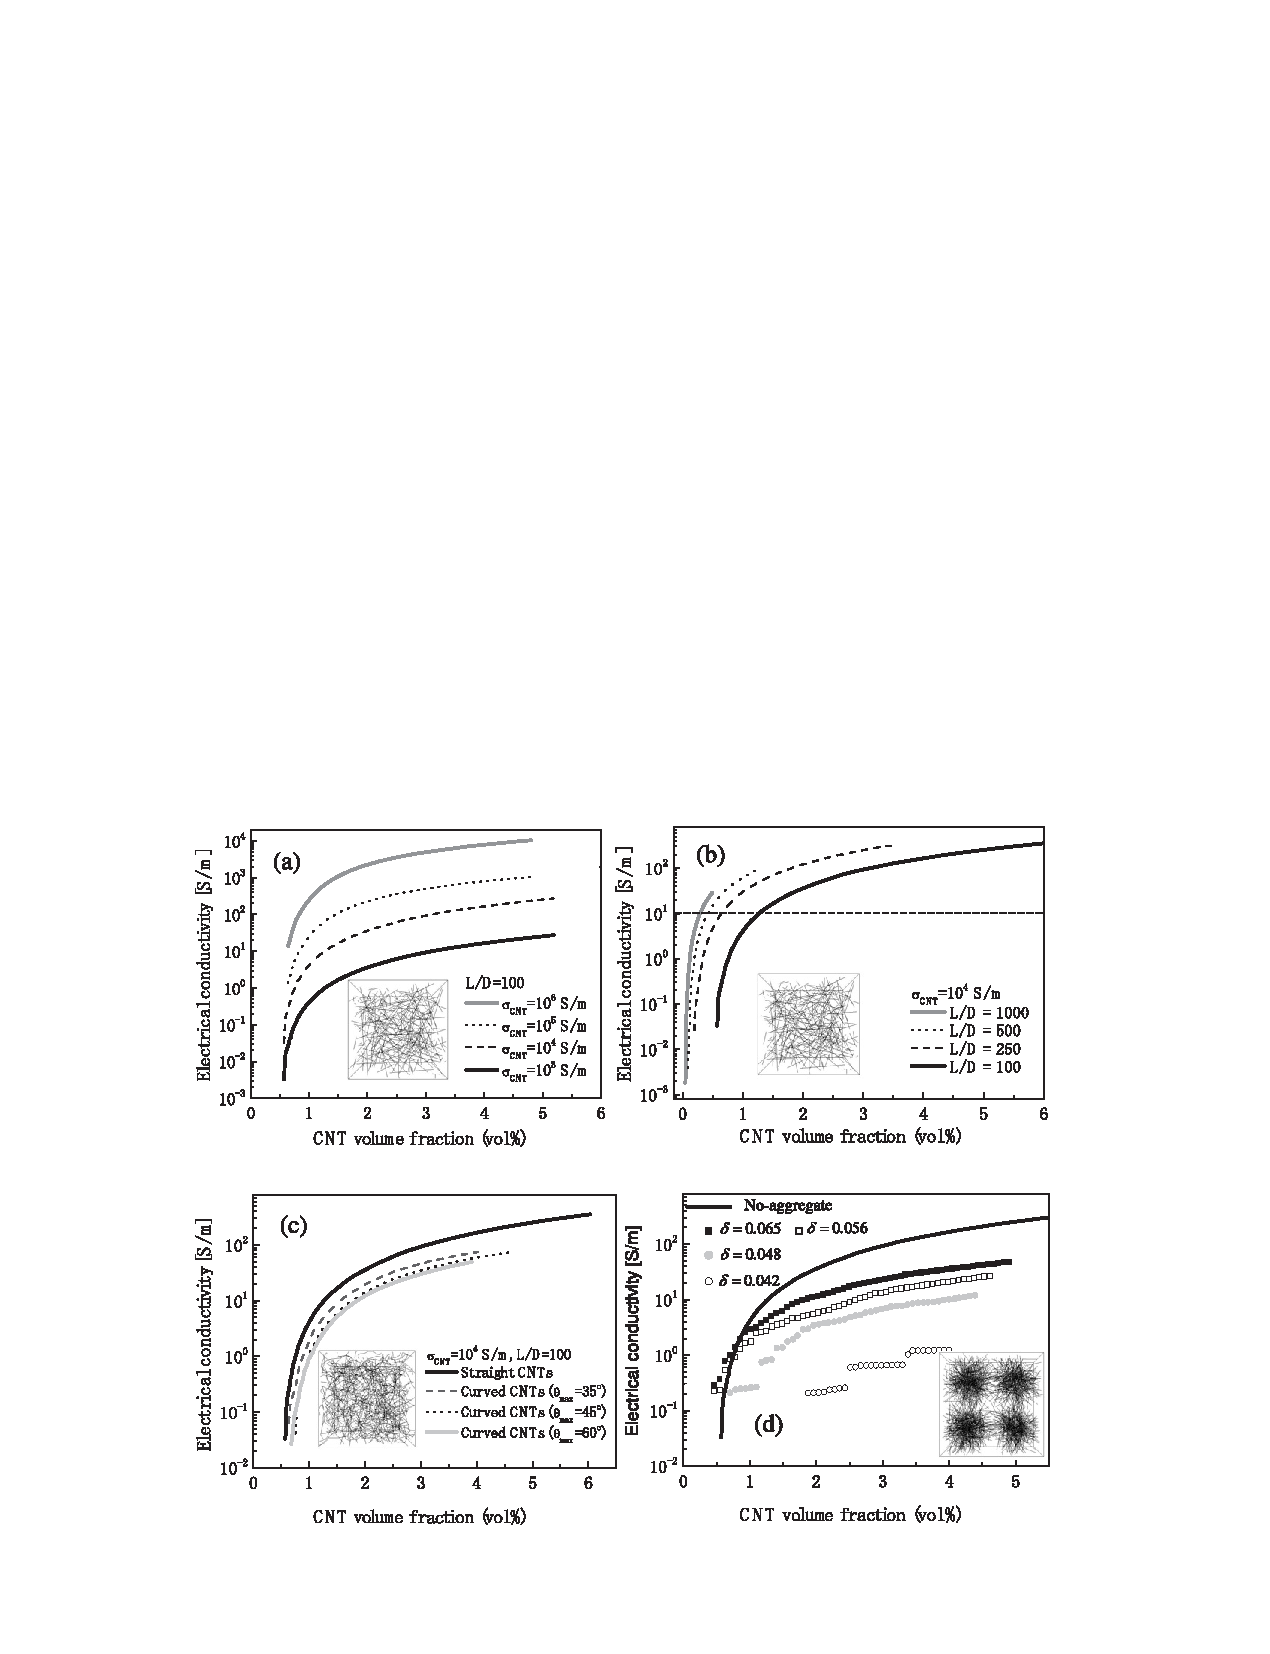
\includegraphics[width=0.9\textwidth]{Hu2008_Fig9.pdf}
	\caption{Effets simulés a) de la conductivité électrique intrinsèque des nanotubes, b) du facteur de forme des nanotubes, c) du niveau de courbure des nanotubes et d) du niveau d'agglomération sur la conductivité électrique des nanocomposites (tirée de \cite{Hu2008}, reproduction avec autorisation)}
	\label{fig:facteurs_geometriques_CNT}
\end{figure}

\FloatBarrier
Les nanotubes de carbone sont principalement produits par décharge d'arc, par ablation laser, par déposition chimique en phase vapeur \cite{Sathyanarayana2013} ou à l'aide de torches au plasma \cite{Kim2009e}. 
Les nanotubes produits peuvent présenter des défauts de cristallinité tels que la présence de pentagones et d'heptagones ou encore des absences dans la structure régulière d'hexagones. 
Ces défauts affectent les propriétés, mais peuvent également être utilisés pour introduire des fonctionnalisations de surface. 

Il est également nécessaire d'ajouter que la conductivité électrique intrinsèque des nanotubes, leur facteur de forme, leur courbure et leur niveau d'agglomération ont tous un impact sur la conductivité électrique des nanocomposites produits (Fig. \ref{fig:facteurs_geometriques_CNT}). 
Un facteur de forme plus élevé permet d'obtenir une conductivité électrique plus élevée et un seuil de percolation plus bas en raison de la résistance électrique de contact non négligeable entre les nanotubes \cite{Hu2008}. 

\subsection{Nanofibres de carbone}

Les nanofibres de carbone partagent un bon nombre de similarités avec les nanotubes de carbone, mais un coût beaucoup plus faible. 
Elles sont produites par déposition chimique en phase vapeur tout comme les nanotubes de carbone. 
Elles peuvent ensuite être graphitisés pour améliorer leur pureté et augmenter leur conductivité électrique \cite{Al-Saleh2009c}. 
La principale différence entre les nanotubes et les nanofibres se situe au niveau de leur morphologie et de leur taille. 
Au lieu d'une structure tubulaire, les nanofibres ont généralement une structure semblable à des bols empilés pour former une série de couches. 
Ces couches superposées peuvent être distinctes ou liées ensemble en spirale \cite{Al-Saleh2009c}. 
Cette structure est distincte des tubes circulaires qui composent les nanotubes. 
Les diamètres des nanofibres sont également légèrement plus grands que pour les nanotubes et se trouvent entre 70 et \SI{200}{\nano\metre}. 
Les propriétés des nanofibres sont similaires à celles des nanotubes de carbone, mais avec un niveau de conductivité électrique réduit. 

\subsection{Graphène}

Les nanoparticules de graphène possèdent la même structure hexagonale d'atomes de carbone que les parois des nanotubes de carbone. 
Cependant, au lieu de former un tube, les atomes forment des couches planes de l'épaisseur d'un seul atome de carbone. 
Ces plans atomiques se superposent pour former des plaquettes pouvant ensuite être séparées par exfoliation. 
Le graphène peut également être intégré à un polymère pour en augmenter la conductivité électrique \cite{Jin2013,Wu2012a,Dweiri2015}. 

\subsection{Combinaison de charges}

Certains auteurs ont tenté de démontrer la présence d'une synergie lorsque des charges de différents facteurs de forme ou tailles sont employées \cite{Kumar2010,Huang2012a,Dweiri2015,Wei2010,Safdari2012}.
Selon les travaux de Kumar, avec une proportion constante de 0,5\% de charges conductrices, la combinaison de nanoplaquettes de graphène et de nanotubes de carbone a obtenu une conductivité électrique supérieure à un nanocomposite composé uniquement de nanoplaquettes de graphène et légèrement supérieure à un nanocomposite avec des nanotubes de carbone uniquement \cite{Kumar2010}. 
Kumar attribue ces résultats au fait que les nanoplaquettes de graĥène agiraient comme une protection des nanotubes durant la mise en forme par ultrasonification en leur permettant de conserver leur facteur de forme et ainsi leur contribution à l'augmentation de la conductivité du nanocomposite. 
Dans ses travaux sur des nanocomposites à matrice d'époxy avec de grandes concentrations de charges, Huang quant à lui dénote l'absence de synergie lorsque le taux de renfort est supérieur à 30\% \cite{Huang2012a}. 
Cependant, d'autres chercheurs présentent des résultats beaucoup plus mitigés \cite{Dweiri2015,Wei2010}. 
Ces derniers dénotent une augmentation de la conductivité lorsqu'une partie des charges de graphène ou de noir de carbone sont remplacées par des nanotubes de carbone. 
Cet effet peut être expliqué simplement par le facteur de forme des nanotubes de carbone qui est beaucoup plus avantageux pour obtenir une structure percolé \cite{Safdari2012}. 
Ainsi, la combinaison de charges conductrices peut parfois être bénéfique, mais il n'existe pas de consensus scientifique quant à la méthode pour généraliser ces résultats. 

\subsection{Méthodes de production des nanocomposites}

Pour tirer profit à l'échelle macroscopique des propriétés des nanomatériaux, il est nécessaire de les mélanger dans une matrice. 
Plusieurs méthodes permettent d'obtenir des mélanges avec les polymères thermoplastiques. 

Une première méthode est la dispersion des nanotubes dans un solvant \cite{Mohammad2006}.
Lors de cette procédure, les nanotubes sont mis en suspension métastable dans un solvant. 
Parla suite, des surfactants sont souvent utilisés pour stabiliser les dispersions de nanoparticules \cite{Huang2012}. 
Cette méthode est appropriée pour les polymères solubles, les polymères à très faible viscosité et pour les monomères \cite{Ma2010}. 
Pour obtenir une distribution homogène, il est nécessaire d'employer un générateur d'ultrasons afin de séparer les agglomérats de nanoparticules. 
On peut évaluer la contrainte en cisaillement ($\sigma_s$) à laquelle sont soumis les agglomérats à l'aide de l'équation suivante dépendant de la viscosité ($\eta$) et de la vitesse de déformation ($\dot{\gamma}$) : 

\begin{equation}
\sigma_s = \eta \dot{\gamma}
\end{equation}

Le brassage par bassin à ultrasons ou à l'aide d'une sonde à ultrasons est une des seules méthodes procurant les contraintes nécessaires pour réduire les agglomérats de nanotubes à simple paroi dans des solvants à faible viscosité (contrainte de \SI[locale=FR]{100}{\mega\pascal}), mais elle peut également induire des dommages et raccourcir les tubes \cite{Huang2012}. 
Cette méthode ne doit donc pas être employée sans considération des propriétés nécessaires pour l'application finale puisque la réduction de la longueur des tubes et les traitements de surface peuvent affecter les propriétés finales \cite{Grossiord2008a, Diez-Pascual2010, Ma2008}.  
Il est à noter que les contraintes nécessaires pour séparer des nanotubes multiparois sont beaucoup plus faible et que d'autres méthodes peuvent les séparer sans induire autant de dommage à leur structure \cite{Huang2012, Ma2010}. 
Un nanotube simple paroi nécessite une contrainte d'approximativement \SI[locale=FR]{100}{\mega\pascal} tandis qu'un nanotube multiparois requiert approximativement \SI[locale=FR]{16}{\kilo\pascal} \cite{Huang2012}. 
Le mélange produit par la mise en solution peut être employé directement ou, si le solvant utilisé est compatible avec le polymère utilisé, il est possible d'obtenir un composite homogène en évaporant le solvant pour conserver les nanoparticules ainsi que le polymère. 

Une seconde méthode de production est le mélange à l'état fondu \cite{Ma2010}. 
Cette méthode est particulièrement applicable aux polymères thermoplastiques, la viscosité résiduelle du polymère induit des efforts de cisaillement avec des contraintes suffisantes pour réduire les agglomérats de nanotubes multiparois (contraintes en cisaillement de \SI[locale=FR]{20}{\kilo\pascal}) \cite{Huang2012}. 
Ce brassage peut s'effectuer avec un mélangeur mécanique ou à l'aide d'une d'extrudeuse. 
Ces deux dernières techniques de brassage ont l'avantage de ne pas causer de dommages aux nanotubes \cite{Ma2010}. 
De plus, la production de nanocomposite par extrusion offre l'avantage de pouvoir atteindre des taux de renfort très élevés \cite{Ma2010}. 

Une autre technique pouvant s'appliquer aux polymères thermoplastiques est le broyage par boulets. 
Ce processus utilise les chocs et le brassage des billes métalliques dans un contenant fermé en rotation pour réduire en poudre les polymères ainsi que les agglomérats de nanotubes.
Cette technique endommage les nanotubes, mais il est possible d'y introduire des composés chimiques pour fonctionnaliser les nanotubes afin de modifier leurs propriétés, par exemple, l'ajout de bicarbonate d'ammonium permet l'obtention de groupes fonctionnels amide et amines améliorant la conductivité électrique des nanotubes \cite{Ma2010, Ma2008a}. 

\begin{table}[]
	\centering
	\caption{Résumé des méthodes de mélange (adapté de \cite{Ma2010})}
	\resizebox{\textwidth}{!}{%
		\begin{tabular}{@{}l p{1.2in} p{2.5in} p{2.75in} @{}}
			\toprule
			Techniques            & Facteurs                    &                                                                                        &                                                                                                     \\
			\cmidrule(l){2-4}     & Endommagement des nanotubes & Types de matrice compatibles                                                           & Principaux paramètres                                                                               \\ \midrule
			Ultrasonification     & Oui                         & Polymère soluble, polymère ou oligomère à faible viscosité, monomère                   & Puissance et mode d'ultrasonification, durée                                                        \\
			Broyage par boulets   & Oui                         & Granules et poudre (polymère ou monomère)                                              & Durée du broyage, vitesse de rotation, taille des boulets, ratio entre les boulets et les nanotubes \\
			Extrusion             & Non                         & Thermoplastiques                                                                       & Température, géométrie et vitesse de rotation de la vis                                             \\
			Mélange par agitation & Non                         & Thermoplastiques, polymère soluble, polymère ou oligomère à faible viscosité, monomère & Taille et géométrie de l'agitateur, vitesse de rotation, temps de mélange                           \\ \bottomrule
		\end{tabular}
	}
	\label{tab:methodes_de_melange}
\end{table}

Les solutions mentionnées précédemment visent à produire des nanocomposites à dispersion homogène dans l'ensemble de la structure. 
Il est également possible de produire des nanocomposites nanostructurés avec une ségrégation des nanocharges qui permet la création d'un réseau continu à une plus petite quantité de nanoparticules \cite{Al-Saleh2011, Li2015a, Deng2014a, Du2011a, Pang2014c, Jia2015}. 
Cette technique peut offrir des composites avec une conductivité électrique beaucoup plus élevée. 
Lors de la fusion de ces polymères, il est cependant possible qu'une diffusion des nanocharges se produise qui affectera drastiquement les propriétés électriques après le changement dans la nanostructure \cite{Wu2012}. 
Ce comportement pourrait d'ailleurs être utilisé comme méthode pour contrôler la puissance dégagée lors du soudage. 

Un des défis lors de la production des nanocomposites est de stabiliser la séparation des nanoparticules qui ont tendance à s’agglomérer.
Cette stabilité peut être atteinte en augmentant l'affinité des nanoparticules avec la matrice d'accueil ou par répulsion entre elles. 
Ces effets peuvent être obtenus par une fonctionnalisation de la surface des nanotubes \cite{Xie2005}. 
La fonctionnalisation peut affecter les propriétés macroscopiques des nanocomposites \cite{Ma2008}. 

\subsection{Conductivité électrique des nanocomposites}

L'ajout de nanoparticules conductrices permet de transformer des polymères non conducteurs en nanocomposites conduisant l'électricité. 
La modification des propriétés électriques est principalement une fonction de la quantité de nanoparticules dispersées, de leur nature, de la qualité de la dispersion, de la nature du polymère et des modifications de surface apportées aux nanoparticules. 

Les variations de la conductivité électrique observées ne peuvent pas être expliquées par la simple loi des mélanges. 
À partir d'une certaine concentration, les nanotubes de carbone forment un réseau continu dans la matrice. 
Cette concentration est nommée seuil de percolation.
En dessous du seuil de percolation, la conductivité du nanocomposite reste à peu près stable et il reste isolant \cite{Bangarusampath2009}. 
Lorsque le réseau est initialement formé, la conductivité électrique du nanocomposite change totalement et une augmentation très rapide de la conductivité électrique, de l'ordre de plusieurs décades, peut être observée. 
Par la suite, la conductivité du nanocomposite continue d'augmenter avec l'ajout de nanoparticules, mais avec une pente beaucoup plus faible. 
L'évolution de la conductivité électrique d'un nanocomposite suit trois régimes distincts qui sont fonction de la concentration en nanocharges conductrices. 
La figure \ref{fig:percolation_electrique} présente une courbe de conductivité électrique en fonction de la concentration en nanotubes de carbone multiparois dans une matrice de PEEK. 
Le facteur de forme \cite{Hu2008}, le niveau de dispersion, l'orientation des particules dans la matrice \cite{Xie2011c} et les traitements de surface sont des facteurs qui ont un impact direct sur le seuil de percolation. 

\begin{figure}[h]
	\centering
	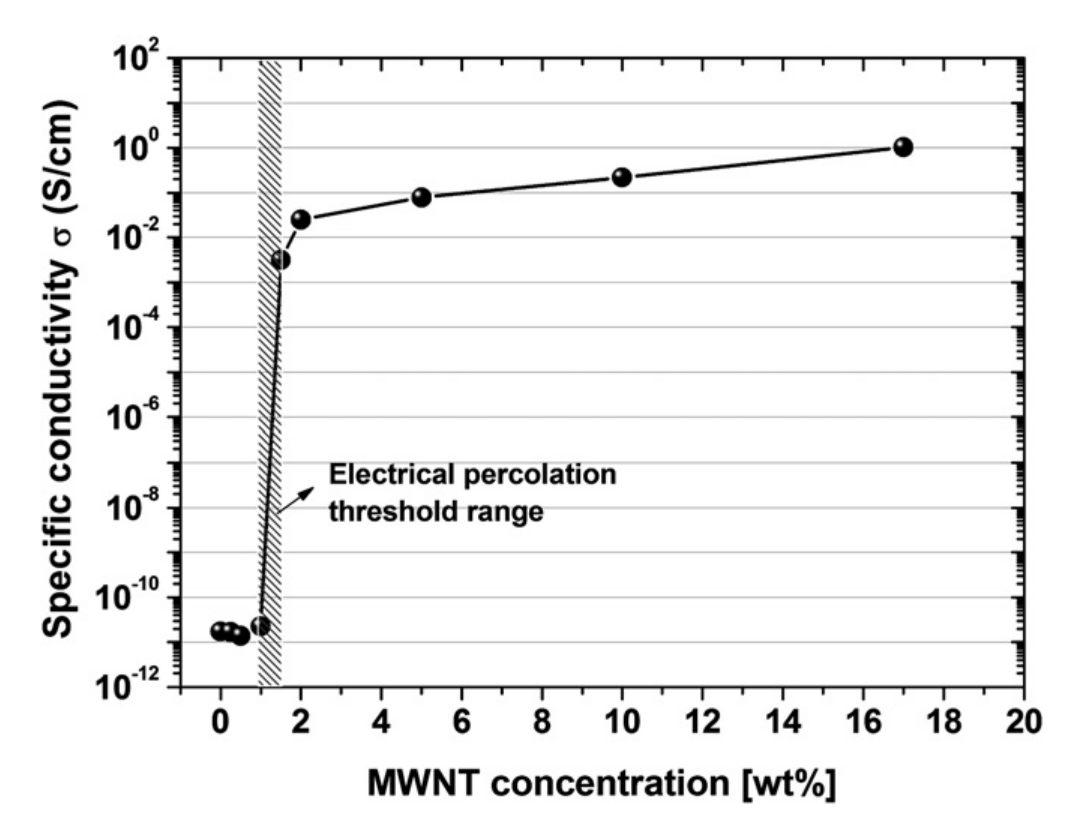
\includegraphics[width=0.7\textwidth]{percolation_electrique.png}
	\caption{Conductivité électrique d'un nanocomposite de PEEK et de nanotubes de carbone (tiré de \cite{Bangarusampath2009}, reproduction avec autorisation)}
	\label{fig:percolation_electrique}
\end{figure}

La plupart des auteurs se concentrent sur la caractérisation du seuil de percolation et peu de mesures de conductivité sont disponibles pour des concentrations élevées de nanotubes. 
Les plus grands gains en conductivité électrique peuvent en effet être observés à ces concentrations et la réduction de la concentration en nanotubes permet de réduire les coûts du matériau. 
Les auteurs rapportent des seuils de percolation variant entre 0,0021\% à 15\% \cite{Bauhofer2009}. 
Une portion des résultats publiés sont résumés à la figure \ref{fig:percolation_articles}. 

\begin{figure}[h]
	\centering
	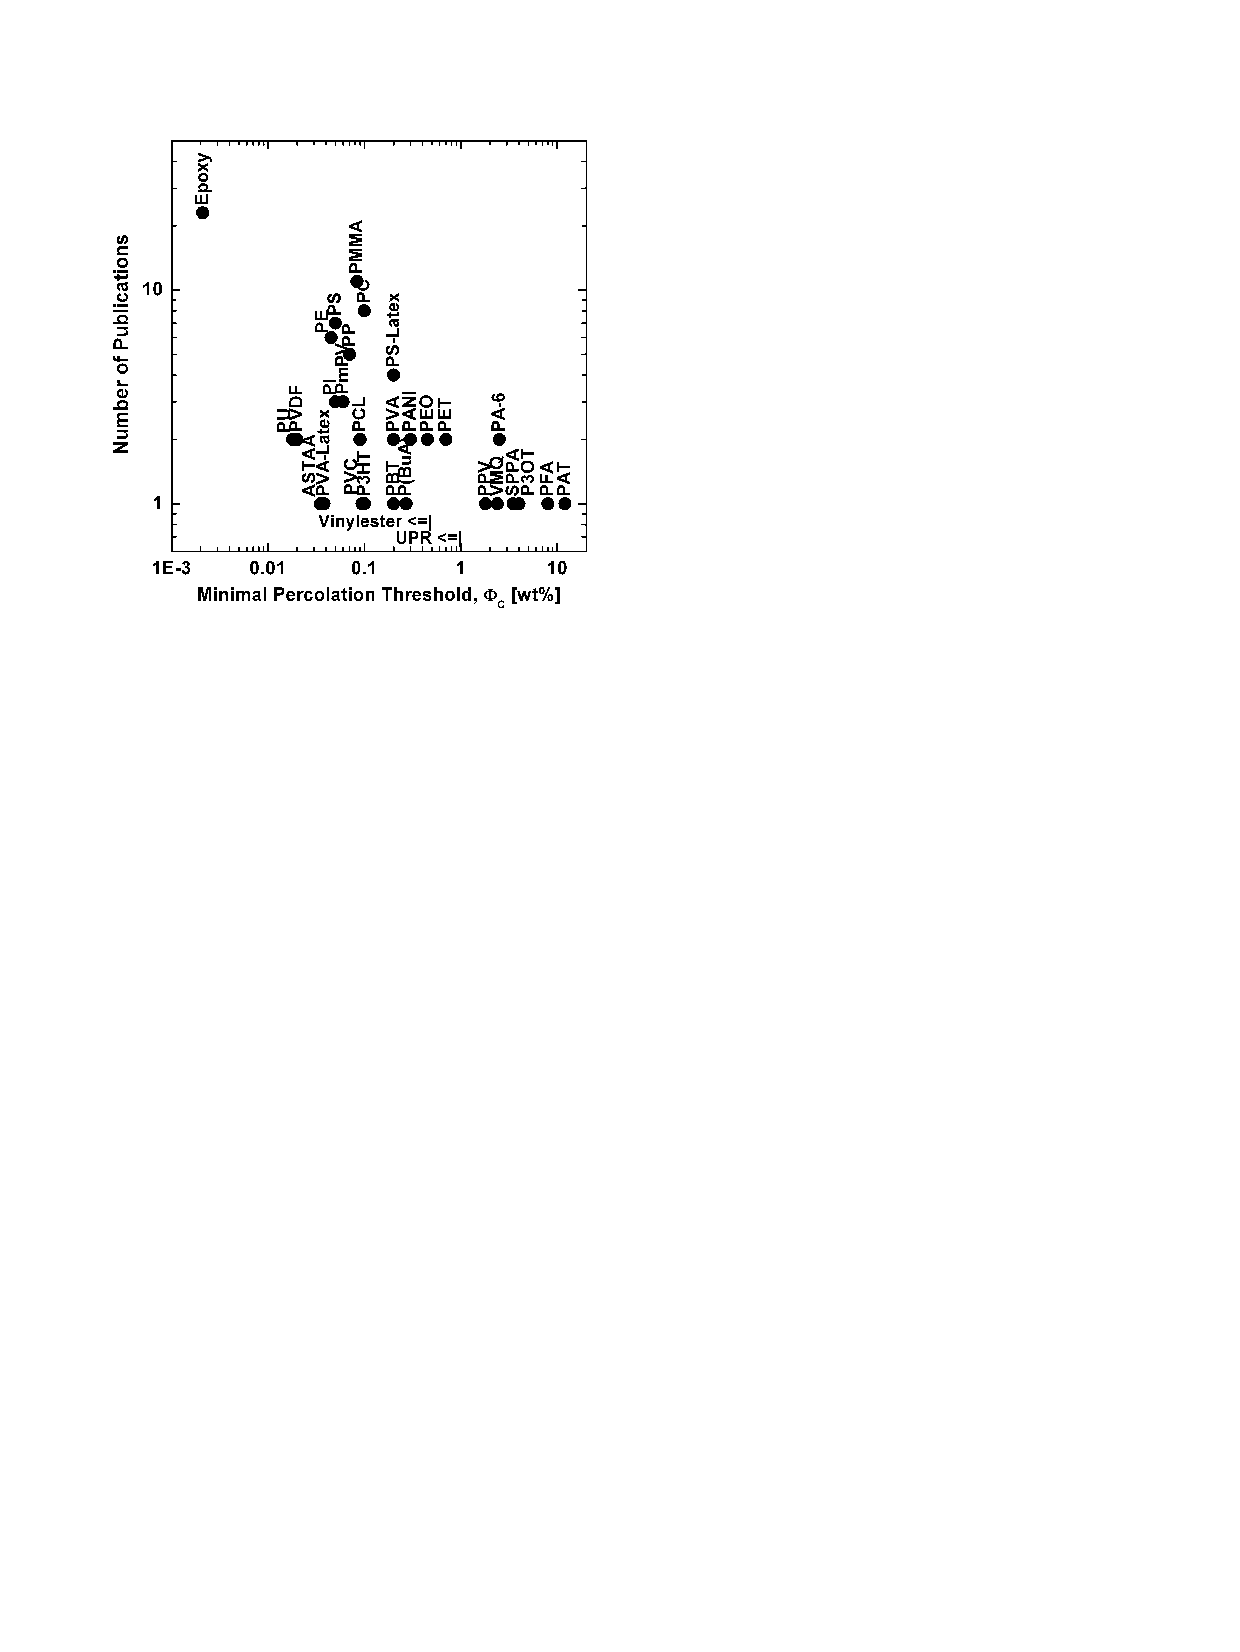
\includegraphics[scale=0.8]{percolation_litterature.pdf}
	\caption{Seuil de percolation minimal reporté et nombre d'articles publiés pour certains systèmes nanocomposites (tiré de \cite{Bauhofer2009}, reproduction avec autorisation)}
	\label{fig:percolation_articles}
\end{figure}

\FloatBarrier
En ce qui concerne l'exploration des concentrations plus élevées de nanoparticules conductrices, quelques articles peuvent être soulignés. 
Par exemple, une conductivité de \SI[locale=FR]{10e4}{\siemens\per\metre} a été atteinte avec une matrice de PMMA et une concentration de 10\% de nanotubes à simple paroi \cite{Bauhofer2009}. 
Pour fin de comparaison, la conductivité électrique de l'acier inoxydable est de \SI[locale=FR]{14.5e5}{\siemens\per\metre} soit une valeur 15 fois plus élevée. 
Malgré quelques rares résultats exceptionnels, l'ensemble des données publiées présente une très grande variabilité, car un grand nombre de facteurs varient entre chaque étude.
Il n'existe aucune courbe maître permettant de généraliser tous ces résultats. 
Le consensus est qu'une bonne dispersion favorise la conductivité électrique \cite{Bauhofer2009} et que les principaux paramètres gouvernant la conductivité sont: 
\begin{inparaenum}
	\item le facteur de forme des nanotubes, 
	\item une bonne dispersion des agglomérats de nanotubes à l'échelle nanométrique et
	\item une distribution uniforme des nanotubes ou des agglomérats à l'échelle microscopique   
\end{inparaenum} \cite{Li2007a}.
Une autre approche pour atteindre le seuil de percolation avec un minimum de charges réside dans la méthode employée pour établir d'un réseau percolé. 
Celui-ci peut s'obtenir de plusieurs façons. 
Il est possible de disperser les nanotubes de façon à obtenir une mauvaise distribution pour maintenir des contacts entre les agrégats \cite{Al-Saleh2009c,Deng2014a}. 
Cette technique vise à produire une structure similaire à ce qui est présenté à la figure \ref{fig:dispersion_distribution}. 
Autrement, il est possible d'obtenir un réseau percolé aux frontières entre des granules en recouvrant leurs surfaces de particules conductrices afin d'obtenir une structure ségrégée \cite{Al-Saleh2011,Pang2014c}. 
Finalement, il est également possible d'employer l'affinité des nanoparticules afin de les disperser préférentiellement dans une seule phase ou à l'interface d'un mélange binaire de polymère \cite{Pang2014c,Deng2014a}. 

\begin{figure}[h]
	\centering
	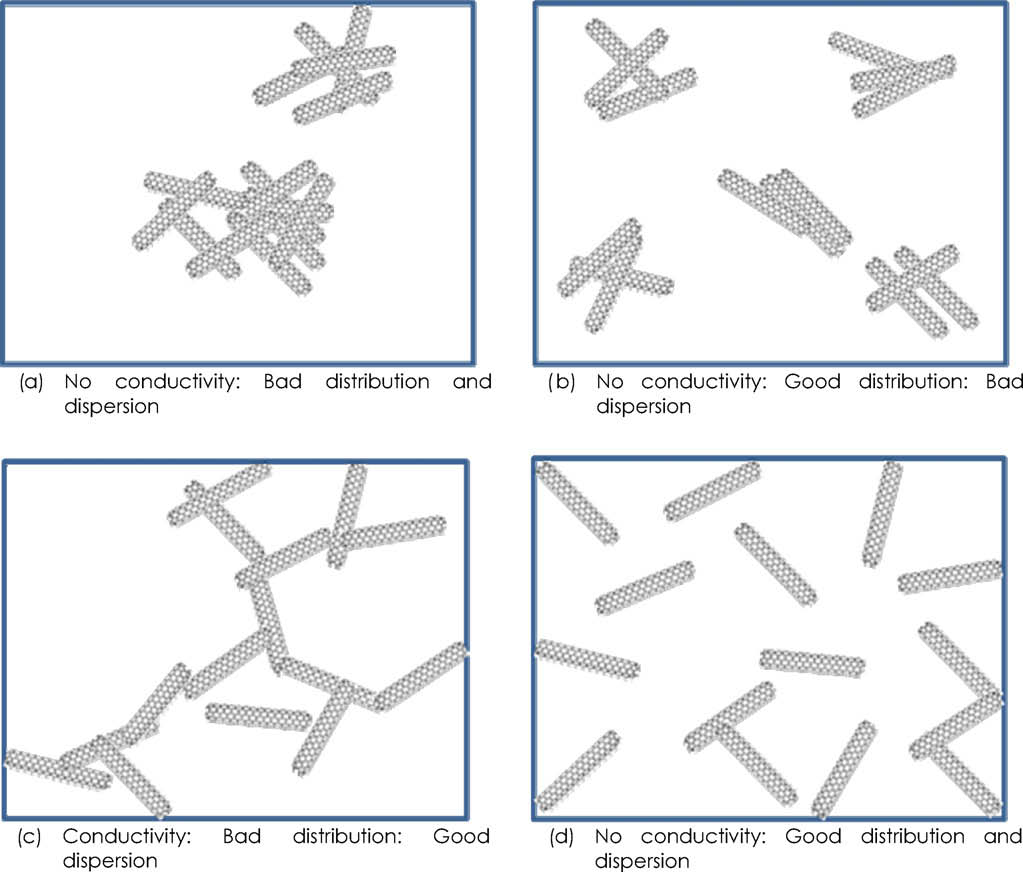
\includegraphics[width=0.6\textwidth]{dispersion_distribution-Al-Saleh2009c.png}
	\caption{Comparaison entre les effets de la distribution et de la dispersion (tiré de \cite{Al-Saleh2009c}, reproduction avec autorisation)}
	\label{fig:dispersion_distribution}
\end{figure}

Également, une fois le seuil de percolation franchi, les conductivités obtenues augmentent moins rapidement que pourrait le suggérer la loi des mélanges. 
Certains travaux \cite{Untereker2009,Cauchy2018} en sont venus à la conclusion que la conductivité électrique obtenue lors du mélange d'une matrice chargée en micro ou nano matériaux est limitée par la résistance de contact élevée entre les particules. 
La dépendance envers la résistance de contact a également été rapportée par d'autres auteurs \cite{Li2007a}. 

La fonctionnalisation des nanotubes est généralement employée pour faciliter leur dispersion, mais elle peut également affecter les propriétés électriques du nanocomposite. 
Certaines modifications vont entraîner une chute de la conductivité électrique tandis que d'autres vont permettre de réduire la résistance de contact. 

\FloatBarrier
Cette variation des effets des divers types de fonctionnalisation par rapport à la conductivité électrique est documentée dans la littérature scientifique. 
Par exemple, il a été démontré que la fonctionnalisation avec des groupes carboxyliques (COOH) produit une réduction très importante de la conductivité \cite{Guadagno2011}. 
Dans cette dernière étude, même en quadruplant la quantité de nanotubes de carbone, les nanotubes fonctionnalisés présentaient une conductivité électrique encore inférieure aux nanotubes non traités. 
La fonctionnalisation avec des groupements amines (NH$_2$) produit également une réduction de la conductivité électrique \cite{Ma2008} et il est postulé que cette réduction est en partie due à la dégradation de la structure des nanotubes nécessaire au dépôt des groupes fonctionnels qui réduit la conductivité des nanotubes sans réduire la résistance de contact \cite{Pandey2012a}.
Même dans le cas de particules métalliques, l'ajout d'une fonctionnalisation à base du composé organique 
1-octanethiol a causé une baisse de la conductivité électrique \cite{Gelves2008a}. 
Au contraire, le dépôt de particules d'argent a pour effet de permettre une réduction de la résistance de contact et ainsi augmente la conductivité électrique  \cite{Ma2010,Cauchy2017}

Les méthodes de fonctionnalisation par enroulement de polymère produisent généralement une réduction de la conductivité électrique \cite{Diez-Pascual2010, Huang2012}. 
Un auteur a cependant obtenu une hausse de la conductivité lorsqu'il a utilisé du polyaniline (PANI), un polymère conducteur, comme agent de revêtement des nanotubes \cite{Vankayala2011}. 
En utilisant un polymère conducteur compatible avec les nanotubes de carbone et avec une matrice de polycaprolactame, l'auteur a pu réduire la résistance de contact tout en améliorant la dispersion des charges. 

Les considérations quant à l'emploi d'un nanocomposite dans le cadre d'un procédé entraînant la fonte de la matrice polymère ne sont pas explorées dans la littérature. 
L'évolution et le maintien de la conductivité lors de la fonte sont des éléments encore inconnus. 
Dans le cas d'un réseau percolé par ségrégation de phase, la diffusion des particules conductrices lors de la fusion pourrait modifier grandement la conductivité électrique du nanocomposite. 

\subsection{Élément chauffant en assemblage de nanoparticules}

Une autre façon d'employer les nanoparticules conductrices pour obtenir un élément chauffant est l'emploi d'un \textit{buckypaper} ou d'un film de nanotubes alignés. 

Le \textit{buckypaper} peut être composé de plusieurs sortes de nanoparticules dont entre autres des nanotubes de carbone ou des nanofibres d'argent. 
Tout comme pour les nanocomposites, un \textit{buckypaper} peut agir comme élément chauffant. 
D'ailleurs, plusieurs chercheurs ont déjà utilisé ce type de solution pour produire des éléments chauffants pouvant servir à dégivrer des surfaces \cite{Pyo2016,Chu2014,Zhang2013}.
Ces chercheurs ont utilisé autant des \textit{buckypaper} de nanotubes de carbone que des feuilles de nanofibres d'argent combinées à un polymère conducteur. 

Pour les films de nanotubes alignés, un film peut être obtenu en enroulant des nanotubes sur un mandrin ou un cadre depuis un substrat sur lequel une forêt de nanotubes a été produite par déposition chimique en phase vapeur. 
Un chercheur a démontré la possibilité d'utiliser un tel film comme système de dégivrage léger pouvant être intégré dans une aile d'avion \cite{Yao2018}.
Une autre équipe quant à elle vient de publier, très récemment, un article dans lequel un film de nanotubes alignés est utilisé pour souder par résistance des échantillons de PEEK \cite{Russello2019}. 
Dans ces travaux, un film de nanotubes positionné entre deux films de PEEK était placé entre les deux extrémités de barreaux de PEEK. 
Une résistance en traction égale à 96\% de celle d'un barreau sans soudure a été obtenue. 

\FloatBarrier
\section{Élastomères thermoplastiques}  

% Définition d'une fonction pour dessiner des structures de polymères
\newcommand\setpolymerdelim[2]{\def\delimleft{#1}\def\delimright{#2}}
\def\makebraces[#1,#2]#3#4#5{%
	\edef\delimhalfdim{\the\dimexpr(#1+#2)/2}%
	\edef\delimvshift{\the\dimexpr(#1-#2)/2}%
	\chemmove{%
		\node[at=(#4),yshift=(\delimvshift)]
		{$\left\delimleft\vrule height\delimhalfdim depth\delimhalfdim
			width0pt\right.$};%
		\node[at=(#5),yshift=(\delimvshift)]
		{$\left.\vrule height\delimhalfdim depth\delimhalfdim
			width0pt\right\delimright_{\rlap{$\scriptstyle#3$}}$};}}
\setpolymerdelim()

Un second concept clé pour la réalisation d'une jonction flexible est en lien avec la nature des élastomères thermoplastiques. 
Les élastomères en général sont une famille de polymère dont la plage de température d'utilisation se situe au-dessus de la température de transition vitreuse. 
Au-delà de celle-ci, les polymères entrent en phase caoutchoutique et les chaînes peuvent commencer à se déplacer et glisser les unes par rapport aux autres. 

\begin{figure}[h]
	\centering
	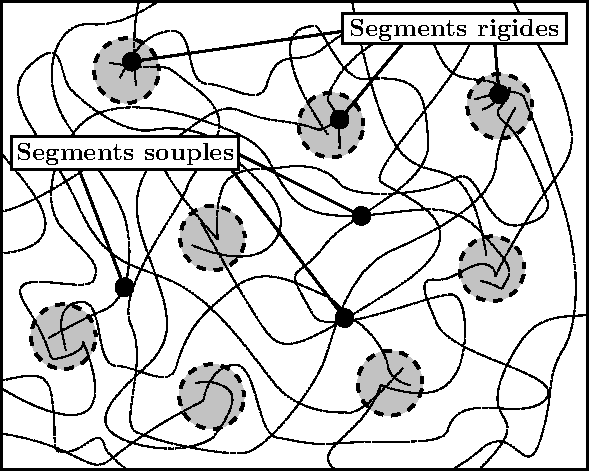
\includegraphics[scale=1]{structure_tribloc.pdf}
	\caption{Exemple de structure pour un élastomère thermoplastique triblocs}
	\label{fig:structure_tribloc}
\end{figure}

Les élastomères commerciaux sont souvent obtenus par une réticulation partielle entre les chaînes de polymères, appelée vulcanisation dans le cas de la transformation du  caoutchouc naturel, ayant pour but de bloquer une partie de la mobilité des chaînes sans pour autant leur retirer leur flexibilité. 
Les élastomères thermoplastiques obtiennent quant à eux ce comportement à l'aide de leur structure et de leur composition. 
Par l'emploi de segments de nature différente, on obtient une structure où les terminaisons composées de segments rigides viennent se lier pour former des blocs à l'intérieur de la structure du matériau \cite{Holden1969}. 
En raison de la faible miscibilité entre les deux polymères causée par une incompatibilité thermodynamique, on observe une ségrégation entre les différentes phases. 
Les blocs rigides, composés de polymère qui sont utilisés sous leur température de transition vitreuse, procurent le même effet que la réticulation entre les chaînes composées, dans leur portion centrale, d'un second polymère utilisé au-dessus de sa température de transition vitreuse \cite{Holden2002}. 
Les blocs rigides sont également capables de fondre une fois chauffés.
On peut ainsi remettre en forme l'élastomère. 

Les élastomères thermoplastiques ont généralement des structures copolymères en triblocs (Fig \ref{fig:polymere_tri_bloc}) ou multiblocs (Fig. \ref{fig:polymere_multi_bloc}). 
Les élastomères copolymères triblocs ont des segments rigides aux deux extrémités. 
Ces dernières sont connectées au travers d'un réseau biphasique dans la structure de l'élastomère (Fig. \ref{fig:structure_tribloc}). 
Contrairement aux élastomères triblocs, figés aux deux extrémités, les élastomères multiblocs utilisent l'enchevêtrement et l'interaction entre les chaînes souples et rigides pour maintenir leur intégrité. 
La présence de segments de polymère semi-cristallins au travers d'une chaîne amorphe permet aux segments cristallins de se lier pour bloquer l'écoulement de la structure (Fig. \ref{fig:structure_TPECryst}). 
Alternativement, dans certains cas, les segments cristallins peuvent également être des segments de polymère amorphe \cite{Holden2002}. 

\vspace{6pt}
\begin{figure}[h]
	\subfigcapskip=6pt
	\centering
	\subfigure[][Structure alternée]
	{\label{fig:polymere_alternee} 								
		\chemfig{\vphantom{B}-[@{op,.75}]A-B-[@{cl,0.25}]}
		\makebraces[5pt,5pt]{\!\!n}{op}{cl}
		\bigskip
	} \quad
	\subfigure[Structure tribloc]
	{\label{fig:polymere_tri_bloc} 					
		\chemfig{
			-[@{opa,.75},,,,opacity=0]A-[@{cla,0.25}]
			-[@{opb,.75}]B-[@{clb,0.25}]
			-[@{opc,.75}]A-[@{clc,0.25},,,,opacity=0]
		}
		\makebraces[5pt,5pt]{\!\!n_{1}}{opa}{cla}
		\makebraces[5pt,5pt]{\!\!n_{2}}{opb}{clb}
		\makebraces[5pt,5pt]{\!\!n_{3}}{opc}{clc}
	} \\ \vspace{6pt}
	\subfigure[Structure multi bloc]
	{\label{fig:polymere_multi_bloc}
		\chemfig{\vphantom{B}
			-[@{op1,.75}]A-[@{cl1,0.25}]
			-[@{op2,.75}]B-[@{cl2,0.25}]
			-[@{op3,.75}]A-[@{cl3,0.25}]
			-[@{op4,.75}]B-[@{cl4,0.25}]
			-[@{op5,.75}]A-[@{cl5,0.25}]
		}
		\makebraces[5pt,5pt]{\!\!n_{i}}{op1}{cl1}
		\makebraces[5pt,5pt]{\!\!n_{i+1}}{op2}{cl2}
		\makebraces[5pt,5pt]{\!\!n_{i+2}}{op3}{cl3}
		\makebraces[5pt,5pt]{\!\!n_{i+3}}{op4}{cl4}
		\makebraces[5pt,5pt]{\!\!n_{i+4}}{op5}{cl5}
		\bigskip
	} 
	\caption{Structures moléculaires de polymères}
	\label{fig:polymere_structure}
\end{figure}

\begin{figure}[h]
	\centering
	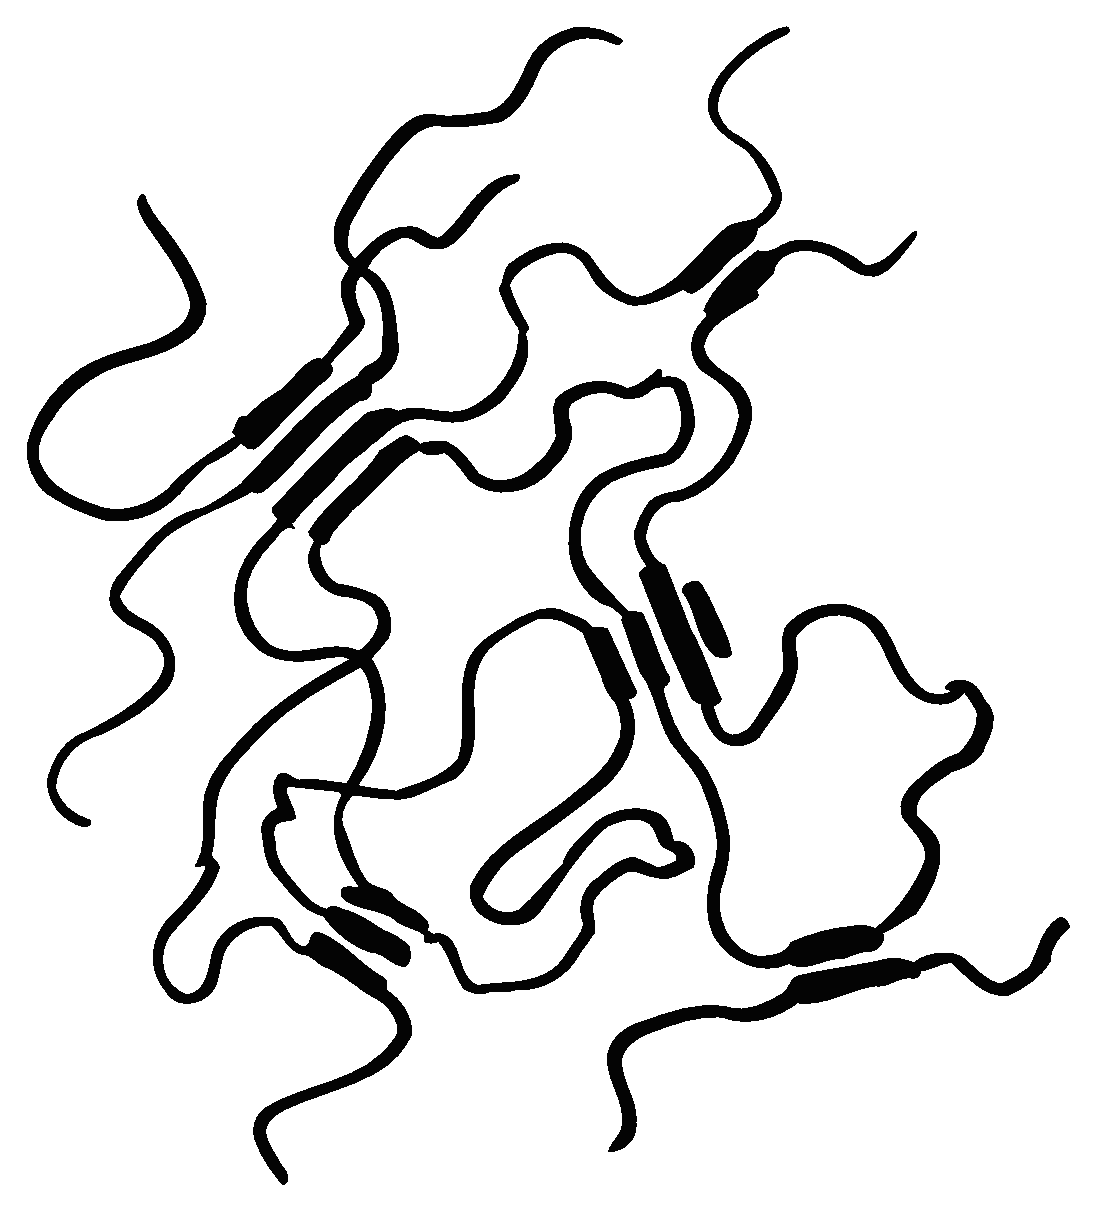
\includegraphics[scale=0.3]{CrystTPE_CC0.pdf}
	\caption{Exemple de structure pour un élastomère thermoplastique avec segments cristallins (image libre de droits)}
	\label{fig:structure_TPECryst}
\end{figure}

\FloatBarrier
En ce qui concerne la soudure des élastomères, très peu de références peuvent être trouvées à ce propos et encore moins en ce qui concerne le soudage entre des matériaux mixtes. 
Un article répertorié documentait le soudage par ultrasons de tissus imprégnés de polyuréthane thermoplastique \cite{Hollande1998}. 
Les soudures présentaient les fibres et l'élastomère comme étant deux phases distinctes l'une de l'autre sans diffusion entre celles-ci. 
Aucun article trouvé ne traitait du soudage où se produisait une diffusion des chaînes dans un autre polymère thermoplastique. 

La solution actuellement employée par ArianeGroup pour les composites à matrice thermodurcissable ne requiert pas l'emploi d'un élastomère thermoplastique. 
Dans ce cas, puisqu'il n'est pas nécessaire de les souder ou de les fondre de nouveau, un élastomère conventionnel avec des chaînes réticulées peut rencontrer les requis techniques. 
Ainsi, un copolymère butadiène-acrylonitrile est présentement collé avec des colles époxydes. 
Les requis techniques du projet sont calqués sur les performances mécaniques de cette solution. 
Cependant, cette méthode présente plusieurs faiblesses. 
Tout d'abord, elle impose un temps de fabrication très long en raison du temps de réticulation de l'époxy. 
En second lieu, elle est très sensible à la présence de contaminants et nécessite une très bonne préparation de surface. 
Finalement, la solution employée n'est pas robuste, elle ne produit pas des résultats totalement répétables en raison de sa sensibilité aux contaminants. 

\section{Enjeux scientifiques}

La revue de la littérature a permis d'identifier une série d'enjeux scientifiques directement liés à cette thèse. 
Tout d'abord, en considérant le contexte du projet qui vise la réalisation d'une jonction entre un composite thermoplastique et un élastomère, il sera nécessaire de considérer la problématique de la compatibilité des polymères et de la diffusion des chaînes entre plusieurs matériaux dissimilaires. 

Également, en considérant le nanocomposite qui sera employé pour le procédé de soudage par résistance, on peut cerner deux enjeux. 
En premier lieu, il y a une grande incertitude quant au comportement électrique d'un nanocomposite conducteur caractérisé à l'état solide une fois rendu à l'état fondu. 
On peut se questionner à savoir si les contacts entre les nanotubes seront maintenus durant la fonte ou si ces liaisons seront affectées et que la conductivité électrique sera perdue. 
En second lieu, lors de l'élaboration d'un nanocomposite conducteur, il peut devenir important de bien contrôler les processus de distribution et de dispersion des charges conductrices dans la matrice polymérique. 




